\documentclass[a4paper,11pt]{book}
%\documentclass[a4paper,twoside,11pt,titlepage]{book}
\usepackage{listings}
\usepackage[utf8]{inputenc}
\usepackage[spanish]{babel}

\usepackage{geometry}
\geometry{a4paper, left=25mm, right=25mm, top=30mm, bottom=30mm}

\usepackage{booktabs} % Para usar \toprule, \midrule y \bottomrule
\usepackage[table,xcdraw]{xcolor} % Colores en la tabla
\addto\captionsspanish{
	\renewcommand{\tablename}{Tabla} % Cambiar "Cuadro" por "Tabla"
}

\usepackage[utf8]{inputenc} % Para codificación UTF-8
\lstset{literate=%
	{á}{{\'a}}1
	{é}{{\'e}}1
	{í}{{\'i}}1
	{ó}{{\'o}}1
	{ú}{{\'u}}1
	{Á}{{\'A}}1
	{É}{{\'E}}1
	{Í}{{\'I}}1
	{Ó}{{\'O}}1
	{Ú}{{\'U}}1
}

\counterwithout{figure}{chapter} % Numeración continua de figuras
\counterwithout{table}{chapter}  % Numeración continua de tablas


\usepackage{listings}
\lstdefinelanguage{yaml}{
	keywords={true,false,null,y,n},
	sensitive=false,
	comment=[l]{\#},
	morecomment=[s]{/*}{*/},
	morestring=[b]',
	morestring=[b]"
}


% \usepackage[style=list, number=none]{glossary} %
%\usepackage{titlesec}
%\usepackage{pailatino}

\decimalpoint
\usepackage{dcolumn}
\newcolumntype{.}{D{.}{\esperiod}{-1}}
\makeatletter
\addto\shorthandsspanish{\let\esperiod\es@period@code}
\makeatother


%\usepackage[chapter]{algorithm}
\RequirePackage{verbatim}
%\RequirePackage[Glenn]{fncychap}
\usepackage{fancyhdr}
\usepackage{graphicx}
\usepackage{afterpage}

\usepackage{longtable}

\usepackage[pdfborder={000}]{hyperref} %referencia

% Diagramas de Gantt
\usepackage{pgfgantt}
\usepackage{xcolor}

% ********************************************************************
% Re-usable information
% ********************************************************************
\newcommand{\myTitle}{Título del proyecto\xspace}
\newcommand{\myDegree}{Grado en Ingeniería Informática\xspace}
\newcommand{\myName}{VIDICAN, MIHNEA IOAN (alumno)\xspace}
\newcommand{\myProf}{GUIRAO MIRAS, JOSÉ MARÍA (tutor1)\xspace}
%\newcommand{\mySupervisor}{Put name here\xspace}
\newcommand{\myFaculty}{Escuela Técnica Superior de Ingenierías Informática y de Telecomunicación\xspace}
\newcommand{\myFacultyShort}{E.T.S. de Ingenierías Informática y de Telecomunicación\xspace}
\newcommand{\myDepartment}{Departamento de Lenguajes y Sistemas Informáticos\xspace}
\newcommand{\myUni}{\protect{Universidad de Granada}\xspace}
\newcommand{\myLocation}{Granada\xspace}
\newcommand{\myTime}{\today\xspace}
\newcommand{\myVersion}{Version 1.0\xspace}


\hypersetup{
pdfauthor = {\myName (email (en) ugr (punto) es)},
pdftitle = {\myTitle},
pdfsubject = {},
pdfkeywords = {palabra_clave1, palabra_clave2, palabra_clave3, ...},
pdfcreator = {LaTeX con el paquete ....},
pdfproducer = {pdflatex}
}

%\hyphenation{}


%\usepackage{doxygen/doxygen}
%\usepackage{pdfpages}
\usepackage{url}
\usepackage{colortbl,longtable}
\usepackage[stable]{footmisc}
%\usepackage{index}

%\makeindex
%\usepackage[style=long, cols=2,border=plain,toc=true,number=none]{glossary}
% \makeglossary

% Definición de comandos que me son tiles:
%\renewcommand{\indexname}{Índice alfabético}
%\renewcommand{\glossaryname}{Glosario}

\pagestyle{fancy}
\fancyhf{}
\fancyhead[LO]{\leftmark}
\fancyhead[RE]{\rightmark}
\fancyhead[RO,LE]{\textbf{\thepage}}
\renewcommand{\chaptermark}[1]{\markboth{\textbf{#1}}{}}
\renewcommand{\sectionmark}[1]{\markright{\textbf{\thesection. #1}}}

\setlength{\headheight}{1.5\headheight}

\newcommand{\HRule}{\rule{\linewidth}{0.5mm}}
%Definimos los tipos teorema, ejemplo y definición podremos usar estos tipos
%simplemente poniendo \begin{teorema} \end{teorema} ...
\newtheorem{teorema}{Teorema}[chapter]
\newtheorem{ejemplo}{Ejemplo}[chapter]
\newtheorem{definicion}{Definición}[chapter]

\definecolor{gray97}{gray}{.97}
\definecolor{gray75}{gray}{.75}
\definecolor{gray45}{gray}{.45}
\definecolor{gray30}{gray}{.94}

\lstset{ frame=Ltb,
     framerule=0.5pt,
     aboveskip=0.5cm,
     framextopmargin=3pt,
     framexbottommargin=3pt,
     framexleftmargin=0.1cm,
     framesep=0pt,
     rulesep=.4pt,
     backgroundcolor=\color{gray97},
     rulesepcolor=\color{black},
     %
     stringstyle=\ttfamily,
     showstringspaces = false,
     basicstyle=\scriptsize\ttfamily,
     commentstyle=\color{gray45},
     keywordstyle=\bfseries,
     %
     numbers=left,
     numbersep=6pt,
     numberstyle=\tiny,
     numberfirstline = false,
     breaklines=true,
   }
 
% minimizar fragmentado de listados
\lstnewenvironment{listing}[1][]
   {\lstset{#1}\pagebreak[0]}{\pagebreak[0]}

\lstdefinestyle{CodigoC}
   {
	basicstyle=\scriptsize,
	frame=single,
	language=C,
	numbers=left
   }
\lstdefinestyle{CodigoC++}
   {
	basicstyle=\small,
	frame=single,
	backgroundcolor=\color{gray30},
	language=C++,
	numbers=left
   }

 
\lstdefinestyle{Consola}
   {basicstyle=\scriptsize\bf\ttfamily,
    backgroundcolor=\color{gray30},
    frame=single,
    numbers=none
   }


\newcommand{\bigrule}{\titlerule[0.5mm]}


%Para conseguir que en las páginas en blanco no ponga cabecerass
\makeatletter
\def\clearpage{%
  \ifvmode
    \ifnum \@dbltopnum =\m@ne
      \ifdim \pagetotal <\topskip
        \hbox{}
      \fi
    \fi
  \fi
  \newpage
  \thispagestyle{empty}
  \write\m@ne{}
  \vbox{}
  \penalty -\@Mi
}
\makeatother

\usepackage{pdfpages}


\begin{document}
\begin{titlepage}
 
 
\newlength{\centeroffset}
\setlength{\centeroffset}{-0.5\oddsidemargin}
\addtolength{\centeroffset}{0.5\evensidemargin}
\thispagestyle{empty}

\noindent\hspace*{\centeroffset}\begin{minipage}{\textwidth}

\centering

\includegraphics[width=0.9\textwidth]{imagenes/logo_ugr.jpg}\\[1.4cm]

\textsc{ \Large TRABAJO FIN DE GRADO\\[0.2cm]}
\textsc{ INGENIERÍA EN ...}\\[1cm]
% Upper part of the page
% 
% Title
{\Huge\bfseries Titulo del Proyecto\\
}
\noindent\rule[-1ex]{\textwidth}{3pt}\\[3.5ex]
{\large\bfseries Subtitulo del Proyecto}
\end{minipage}

\vspace{2.5cm}
\noindent\hspace*{\centeroffset}\begin{minipage}{\textwidth}
\centering

\textbf{Autor}\\ {Nombre Apellido1 Apellido2 (alumno)}\\[2.5ex]
\textbf{Directores}\\
{Nombre Apellido1 Apellido2 (tutor1)\\
Nombre Apellido1 Apellido2 (tutor2)}\\[2cm]

\includegraphics[width=0.3\textwidth]{imagenes/etsiit_logo.png}\\[0.1cm]
\textsc{Escuela Técnica Superior de Ingenierías Informática y de Telecomunicación}\\
\textsc{---}\\
Granada, mes de 201
\end{minipage}
%\addtolength{\textwidth}{\centeroffset}
%\vspace{\stretch{2}}
\end{titlepage}



\chapter*{}
%\thispagestyle{empty}
%\cleardoublepage

%\thispagestyle{empty}

\begin{titlepage}
 
 
\setlength{\centeroffset}{-0.5\oddsidemargin}
\addtolength{\centeroffset}{0.5\evensidemargin}
\thispagestyle{empty}

\noindent\hspace*{\centeroffset}\begin{minipage}{\textwidth}

\centering
%
\includegraphics[width=0.9\textwidth]{imagenes/logo_ugr.jpg}\\[1.4cm]

%\textsc{ \Large PROYECTO FIN DE CARRERA\\[0.2cm]}
%\textsc{ INGENIERÍA EN INFORMÁTICA}\\[1cm]
% Upper part of the page
% 

 \vspace{3.3cm}

%si el proyecto tiene logo poner aquí

\includegraphics{imagenes/logo.png} 
 \vspace{0.5cm}

% Title

{\Huge\bfseries Título del proyecto\\
}
\noindent\rule[-1ex]{\textwidth}{3pt}\\[3.5ex]
{\large\bfseries Subtítulo del proyecto.\\[4cm]}
\end{minipage}

\vspace{2.5cm}
\noindent\hspace*{\centeroffset}\begin{minipage}{\textwidth}
\centering

\textbf{Autor}\\ {Nombre Apellido1 Apellido2 (alumno)}\\[2.5ex]
\textbf{Directores}\\
{Nombre Apellido1 Apellido2 (tutor1)\\
Nombre Apellido1 Apellido2 (tutor2)}\\[2cm]
%
\includegraphics[width=0.15\textwidth]{imagenes/tstc.png}\\[0.1cm]
%\textsc{Departamento de Teoría de la Señal, Telemática y Comunicaciones}\\
%\textsc{---}\\
%Granada, mes de 201
\end{minipage}
%\addtolength{\textwidth}{\centeroffset}
\vspace{\stretch{2}}

 
\end{titlepage}





\thispagestyle{empty}

\begin{center}
{\large\bfseries Título del Proyecto: Subtítulo del proyecto}\\
\end{center}
\begin{center}
Nombre Apellido1 Apellido2 (alumno)\\
\end{center}

%\vspace{0.7cm}
\noindent{\textbf{Palabras clave}: palabra\_clave1, palabra\_clave2, palabra\_clave3, ......}\\

\vspace{0.7cm}
\noindent{\textbf{Resumen}}\\

Poner aquí el resumen.
\cleardoublepage


\thispagestyle{empty}


\begin{center}
{\large\bfseries Project Title: Project Subtitle}\\
\end{center}
\begin{center}
First name, Family name (student)\\
\end{center}

%\vspace{0.7cm}
\noindent{\textbf{Keywords}: Keyword1, Keyword2, Keyword3, ....} \\

\vspace{0.7cm}
\noindent{\textbf{Abstract}}\\

Write here the abstract in English.

\chapter*{}
\thispagestyle{empty}

\noindent\rule[-1ex]{\textwidth}{2pt}\\[4.5ex]

Yo, \textbf{Nombre Apellido1 Apellido2}, alumno de la titulación TITULACIÓN de la \textbf{Escuela Técnica Superior
de Ingenierías Informática y de Telecomunicación de la Universidad de Granada}, con DNI XXXXXXXXX, autorizo la
ubicación de la siguiente copia de mi Trabajo Fin de Grado en la biblioteca del centro para que pueda ser
consultada por las personas que lo deseen.

\vspace{6cm}

\noindent Fdo: Nombre Apellido1 Apellido2

\vspace{2cm}

\begin{flushright}
Granada a X de mes de 201 .
\end{flushright}


\chapter*{}
\thispagestyle{empty}

\noindent\rule[-1ex]{\textwidth}{2pt}\\[4.5ex]

D. \textbf{Nombre Apellido1 Apellido2 (tutor1)}, Profesor del Área de XXXX del Departamento YYYY de la Universidad de Granada.

\vspace{0.5cm}

D. \textbf{Nombre Apellido1 Apellido2 (tutor2)}, Profesor del Área de XXXX del Departamento YYYY de la Universidad de Granada.


\vspace{0.5cm}

\textbf{Informan:}

\vspace{0.5cm}

Que el presente trabajo, titulado \textit{\textbf{Título del proyecto, Subtítulo del proyecto}},
ha sido realizado bajo su supervisión por \textbf{Nombre Apellido1 Apellido2 (alumno)}, y autorizamos la defensa de dicho trabajo ante el tribunal
que corresponda.

\vspace{0.5cm}

Y para que conste, expiden y firman el presente informe en Granada a X de mes de 201 .

\vspace{1cm}

\textbf{Los directores:}

\vspace{5cm}

\noindent \textbf{Nombre Apellido1 Apellido2 (tutor1) \ \ \ \ \ Nombre Apellido1 Apellido2 (tutor2)}

\chapter*{Agradecimientos}
\thispagestyle{empty}

       \vspace{1cm}


Poner aquí agradecimientos...


\frontmatter
\tableofcontents
\listoffigures

\listoftables
%
\mainmatter
\setlength{\parskip}{5pt}

\chapter{Introducción}

La adherencia terapéutica hace referencia al grado de concordancia entre el comportamiento de un paciente y las instrucciones y/o recomendaciones recibidas por parte de un profesional de salud en cuanto a la toma de medicamentos, la implementación de cambios dietéticos y de estilo de vida. Esta adherencia resulta crítica tanto para asegurar la eficacia de los tratamientos, así como para optimizar los resultados de salud y minimizar los riesgos asociados a la morbilidad y resistencia a los mismos. 

La labor de seguimiento supone un proceso interactivo entre el farmacéutico y el paciente, por ello, el rol de este último será de vital importancia para una correcta gestión del tratamiento en vigor.



 \cite{pages2018metodos}

%%%%%%%%%%%%%%%%%%%%%%%%%%%%%%%%%%%%%%%%%%%%%%%%%%%%%%%%%%%%%%%%
\section{Problema a resolver}



Es por ello por lo que el proyecto tiene como fin mejorar dicha adherencia mediante el desarrollo de una plataforma para facilitar a los farmacéuticos la elaboración, preparación y seguimiento de la medicación para pacientes, así como la recomendación y advertencia sobre la toma de la misma de acuerdo a directrices específicas. 



%%%%%%%%%%%%%%%%%%%%%%%%%%%%%%%%%%%%%%%%%%%%%%%%%%%%%%%%%%%%%%%%
\section{Estado del arte}

%%%%%%%%%%%%%%%%%%%%%%%%%%%%%%%%%%%%%%%%%%%%%%%%%%%%%%%%%%%%%%%%
\section{Objetivos}

%
\chapter{Análisis y especificaciones del proyecto}

En la base de todo proyecto informático reside una idea concreta acompañada de objetivos específicos que se desean alcanzar. Para cumplir con lo propuesto, resulta necesario establecer un punto de partida que desarrolle detalladamente dicha idea. Este proceso incluye la identificación de los actores que intervendrán en el proyecto y la comprensión de sus necesidades, las cuales serán aspectos a tener en cuenta para la consecución del producto deseado.

%%%%%%%%%%%%%%%%%%%%%%%%%%%%%%%%%%%%%%%%%%%%%%%%%%%%%%%%%%%%%%%%%%%
\section{Identificación de actores}
Se definen tres categorías de actores:
\begin{itemize}
	\item \textbf{Personal sanitario.} Dado que este proyecto está orientado de forma exclusiva a farmacias comunitarias\footnote{Las farmacias comunitarias son establecimientos sanitarios de carácter privado pero de interés público donde el farmacéutico titular-propietario, asistido, en su caso, de ayudantes o auxiliares, presta servicios básicos a la población: dispensación de los medicamentos y productos sanitarios, control y custodia de las recetas médicas dispensadas, seguimiento de los tratamientos farmacológicos y no farmacológicos a los pacientes, entre otros. \cite{Ley16_1997}}, se distinguen los siguientes tipos de personal sanitario:
	\begin{itemize}
		\item \textbf{Farmacéutico.} Es la persona cualificada y encargada para elaborar y dispensar medicación, recomendar la implantación de hábitos de vida, dietas, controlar las recetas médicas dispensadas y realizar un seguimiento del tratamiento en los pacientes con el fin de determinar la adherencia y ofrecer recomendaciones para mejorarla. A los farmacéuticos se les atribuye más tareas y cargos dentro de una oficina de farmacia, pero las  funciones anteriores serán las principales para el desarrollo de este proyecto.
		
		\item \textbf{Técnico de farmacia.} Es una persona con formación en el campo de la farmacia que asiste al farmacéutico titular en diferentes tareas: dispensación de productos farmacéuticos junto con sus indicaciones de uso, toma de constantes vitales, bajo la supervisión del facultativo, y parámetros somatométricos (como el peso y la altura), además de realizar tareas administrativas.
	\end{itemize}

	\item \textbf{Clientes.} En esta categoría existen dos perfiles:
	\begin{itemize}
		\item \textbf{Paciente.} Se trata del individuo que busca atención o recibe cuidados de salud debido a enfermedades, lesiones, para mejorar su bienestar, para prevenir otras enfermedades o para obtener diagnósticos sobre su estado de salud. \cite{UniNavarra}
		
		\item \textbf{Tutor o acompañante del paciente}. En el caso en que el paciente no sea una persona independiente, como un menor o un anciano, será el tutor, representante o acompañante del mismo quien realizará todas las tareas de recogida de mediación y de proporción de información en su lugar.
	\end{itemize}

	\item \textbf{Administrador del sistema.} Será el encargado de llevar a cabo tareas de monitorización de la actividad de la plataforma final, ofrecer soporte y manejar la creación y eliminación de oficinas de farmacia dentro del proyecto. 
\end{itemize}

%%%%%%%%%%%%%%%%%%%%%%%%%%%%%%%%%%%%%%%%%%%%%%%%%%%%%%%%%%%%%%%%%%%
\section{Historias de usuario}
Las historias de usuario en el desarrollo de software son descripciones informales expresadas en lenguaje natural sobre una o varias acciones que un actor desea realizar y su justificación. Sirven como referencia para crear un requisito que deberá cumplir el sistema final. 

Para este proyecto se detallan las siguientes historias de usuario, las cuales irán nombradas de la forma HU-XX, siendo XX el número de historia en orden creciente:

\begin{itemize}
	\item \textbf{HU-01: Farmacéutico.} El farmacéutico titular de una farmacia atiende a una variedad de clientes a lo largo de un día. La mayoría de ellos acude a recoger la medicación prescrita, otros para que se les dispense una medicación personalizada y algunos llegan para aclarar sus dudas o incertidumbres sobre la toma de medicamentos y comunicar sus avances en cuanto a todo tipo de tratamientos. El farmacéutico despacha a todas las personas de igual manera, aunque emplea un mayor tiempo en aquellas consultas más complejas, como es el caso del seguimiento de un tratamiento, su cumplimiento o el estudio del uso individualizado de los medicamentos, con el propósito de detectar reacciones adversas que puedan producirse. Para poder ser más eficiente en su jornada laboral, requiere que muchas de estas tareas se automaticen, pues algunos de los datos que recoge manualmente son de carácter estadístico y no se precisa su presencia obligatoria.
	
	\item \textbf{HU-02: Técnico de farmacia.} El técnico de farmacia es añadido a una farmacia por su farmacéutico titular y no tiene las mismas responsabilidades que el este, pero también puede dispensar medicamentos y atender consultas de los pacientes sobre sus tratamientos en curso. El farmacéutico delega en el técnico varias funciones, como contribuir al análisis del cumplimiento de tratamientos, dietas o hábitos de vida, y medir constantes vitales y parámetros somatométricos. Además, el técnico es responsable de registrar a los pacientes en el sistema de la farmacia, 
	
	\item \textbf{HU-03. Paciente.} Un paciente llega a la farmacia para retirar su medicación recetada. Tras comenzar el tratamiento, puede regresar para que se le dispense nuevamente el medicamento necesario o para realizar un seguimiento de su tratamiento o hábito prescrito. Sin embargo, en algunas ocasiones no es necesaria la dispensación de nueva medicación y el paciente sólo necesita informar sobre el cumplimiento de lo prescrito. Estas tareas son algo que el paciente puede, y a menudo prefiere, realizar desde su domicilio, sin necesidad de acudir presencialmente a la farmacia.
	
	\item \textbf{HU-03. Acompañante del paciente.} Un paciente menor de edad debe informar sobre su estado de salud unos días después de iniciar su tratamiento. Sin embargo, debido a su corta edad, son sus padres quienes deben realizar esta tarea, ya que el menor no puede acudir solo a la farmacia. Los padres preferirían que esta gestión pudiera realizarse desde su domicilio o desde cualquier lugar donde se encuentren, ya que es posible que estén lejos de la farmacia donde registraron el inicio del tratamiento.

\end{itemize}


%%%%%%%%%%%%%%%%%%%%%%%%%%%%%%%%%%%%%%%%%%%%%%%%%%%%%%%%%%%%%%%%%%%
\section{Requisitos}
Los requisitos son especificaciones que el sistema debe cumplir para satisfacer las necesidades de los usuarios finales. El objetivo que plantean es guiar el diseño, el desarrollo y las pruebas y mantenimiento del software. 

%%%%%%%%%%%%%%%%%%%%%%%%%%%%%%%%%%%%%%%%%%%%%%%%%%%%%%%%%%%%%%%%%%%
\subsection{Requisitos funcionales}
Los requisitos funcionales especifican lo que debe realizar el sistema en cuanto a funciones o servicios. Los que se listan a continuación vienen nombrados por RFXX, donde XX es el número del requisito en orden creciente.

\begin{itemize}
	\item \textbf{RF1: Registro de pacientes.} El sistema permitirá al personal sanitario registrar pacientes en la farmacia.
	
	\begin{itemize}
		 
		\item \textbf{RF1.1}: El farmacéutico y el técnico de farmacia podrán registrar nuevos pacientes en el sistema.
		\item \textbf{RF1.2}: El sistema permitirá al farmacéutico y al técnico de farmacia actualizar la información de pacientes existentes.
		\item \textbf{RF1.3}: El sistema permitirá registrar la información de contacto del tutor o acompañante del paciente, en caso de que el paciente sea un menor o una persona dependiente.
	\end{itemize}

	\item \textbf{RF2: Dispensación de medicamentos.} El sistema permitirá la dispensación de medicamentos recetados a los pacientes.
	
	\begin{itemize}
		\item \textbf{RF2.1}: El farmacéutico podrá registrar la dispensación de medicamentos recetados a los pacientes.
		\item \textbf{RF2.2}: El técnico de farmacia podrá asistir en la dispensación de medicamentos, bajo la supervisión del farmacéutico.
		\item \textbf{RF2.3}: El sistema registrará la fecha y hora de cada dispensación, así como la identidad del personal que realizó la dispensación.
	\end{itemize}
	
	\item \textbf{RF3: Análisis de la adherencia.} El sistema permitirá al personal sanitario realizar el seguimiento de los tratamientos de los pacientes para determinar el nivel de adherencia.
	
	\begin{itemize}
		\item \textbf{RF3.1}: El farmacéutico podrá registrar observaciones sobre el progreso del tratamiento de un paciente.
		\item \textbf{RF3.2}: El técnico de farmacia podrá ingresar datos de seguimiento como constantes vitales y parámetros somatométricos del paciente.
		\item \textbf{RF3.3}: El paciente, o su tutor o acompañante, podrá ingresar datos de sequimiento de un tratamiento y notificar problemas surgidos en el sistema.
		\item \textbf{RF3.4}: El sistema generará alertas y recordatorios para el seguimiento de tratamientos a pacientes con condiciones críticas o crónicas.
		\item \textbf{RF3.5}: El sistema realizará un análisis del seguimiento del tratamiento e informará sobre las estadísticas obtenidas para determinar el grado de adherencia 
	\end{itemize}
	
	\item \textbf{RF4: Consulta de información médica.} El sistema permitirá al personal sanitario y a los pacientes consultar información sobre los tratamientos y medicamentos.
	
	\begin{itemize}
		\item \textbf{RF4.1}: El farmacéutico podrá consultar el historial de tratamiento de un paciente.
		\item \textbf{RF4.2}: El técnico de farmacia podrá acceder a la información relevante para la dispensación y seguimiento del tratamiento, bajo la supervisión del farmacéutico.
		\item \textbf{RF4.3}: El paciente podrá consultar su historial de medicación y tratamiento en el sistema.
		\item \textbf{RF4.4}: El acompañante del paciente, en caso de ser un menor o dependiente, podrá acceder a la información médica del paciente mediante un acceso autorizado.
	\end{itemize}
	
	\item \textbf{RF5: Automatización de tareas administrativas.} El sistema automatizará ciertas tareas administrativas para mejorar la eficiencia del personal sanitario.
	
	\begin{itemize}
		\item \textbf{RF5.1}: El sistema automatizará la generación de informes estadísticos sobre la dispensación de medicamentos.
		\item \textbf{RF5.2}: El sistema permitirá la programación automática de seguimientos para tratamientos continuos o crónicos.
	\end{itemize}
	
	\item \textbf{RF6: Gestión de usuarios del sistema.} El sistema permitirá la gestión de usuarios, incluyendo la creación, modificación y eliminación de cuentas para el personal sanitario y administrativo.
	
	\begin{itemize}
		\item \textbf{RF6.1}: El administrador del sistema podrá crear, modificar y eliminar cuentas de usuarios para farmacéuticos y técnicos de farmacia.
		\item \textbf{RF6.2}: El sistema permitirá asignar roles y permisos específicos según el perfil del usuario.
	\end{itemize}
	
	\item \textbf{RF7: Seguimiento de tratamientos no farmacológicos.} El sistema permitirá al personal sanitario registrar y realizar el seguimiento de tratamientos no farmacológicos.
	
	\begin{itemize}
		\item \textbf{RF7.1}: El farmacéutico podrá registrar recomendaciones de hábitos de vida saludables, como dietas, ejercicio físico, y otros tratamientos no farmacológicos.
		\item \textbf{RF7.2}: El técnico de farmacia podrá asistir en el seguimiento del cumplimiento de estos hábitos de vida por parte del paciente.
		\item \textbf{RF7.3}: El sistema permitirá al paciente o su tutor registrar su progreso en la adopción de estos hábitos de vida en el mismo.
		\item \textbf{RF7.4}: El sistema generará alertas o recordatorios para el paciente sobre el cumplimiento de los tratamientos no farmacológicos, como recordar la realización de ejercicios o adherencia a una dieta específica.
	\end{itemize}

\end{itemize}

%%%%%%%%%%%%%%%%%%%%%%%%%%%%%%%%%%%%%%%%%%%%%%%%%%%%%%%%%%%%%%%%%%%
\subsection{Requisitos no funcionales}

\begin{itemize}
	\item \textbf{RFN1: Seguridad de la información.} El sistema garantizará la seguridad y confidencialidad de la información médica y personal de los pacientes.
	
	\begin{itemize}
		\item \textbf{RFN1.1}: El sistema utilizará un cifrado seguro para proteger los datos sensibles almacenados y transmitidos.
		\item \textbf{RFN1.2}: Solo el personal autorizado, como farmacéuticos, técnicos de farmacia, y administradores del sistema, tendrán acceso a la información médica y personal de los pacientes. Los pacientes también tendrán acceso a dicha información, pero no podrán consultar la información de otros pacientes si no son tutores o acompañantes autorizados.
		\item \textbf{RFN1.3}: El sistema requerirá autenticación para acceder a funciones administrativas o a información confidencial.
	\end{itemize}
	
	\item \textbf{RFN2: Disponibilidad del sistema.} El sistema deberá estar disponible para su uso en las farmacias comunitarias en todo momento.
	
	\begin{itemize}
		\item \textbf{RFN2.1}: El sistema garantizará una alta disponibilidad para asegurar que los servicios no se vean interrumpidos durante el horario de atención de las farmacias.
		\item \textbf{RFN2.2}: El sistema deberá contar con mecanismos de respaldo y recuperación ante fallos o desastres, para minimizar el tiempo de inactividad.
	\end{itemize}
	
	\item \textbf{RFN3: Rendimiento.} El sistema deberá ser capaz de manejar un alto volumen de transacciones y consultas sin afectar su rendimiento.
	
	\begin{itemize}
		\item \textbf{RFN3.1}: El sistema deberá procesar la dispensación de medicamentos y la asignación de tratamientos no farmacológicos en un tiempo mínimo por transacción.
		\item \textbf{RFN3.2}: El sistema deberá soportar la gestión simultánea de un número elevado de usuarios sin degradación en el rendimiento.
	\end{itemize}
	
	\item \textbf{RFN4: Usabilidad.} El sistema deberá ser fácil de usar para todo el personal sanitario, considerando su nivel de familiaridad con las tecnologías.
	
	\begin{itemize}
		\item \textbf{RFN4.1}: La interfaz de usuario deberá ser intuitiva, permitiendo a los usuarios realizar con fluidez sus tareas.
		\item \textbf{RFN4.3}: El sistema deberá ser compatible con una amplia gama de dispositivos, permitiendo a los usuarios acceder a sus funciones de manera flexible y desde cualquier lugar.
	\end{itemize}
	
	\item \textbf{RFN5: Escalabilidad.} El sistema deberá ser escalable para adaptarse al crecimiento del número de usuarios y farmacias integradas.
	
	\begin{itemize}
		\item \textbf{RFN5.1}: El sistema deberá poder integrar nuevas farmacias comunitarias sin necesidad de interrupciones en el servicio.
		\item \textbf{RFN5.2}: El sistema deberá poder integrar nuevo personal sanitarios y nuevos pacientes sin necesidad de interrupciones en el servicio.
	\end{itemize}
	
	\item \textbf{RFN6: Cumplimiento normativo.} El sistema deberá cumplir con todas las normativas y regulaciones vigentes en el sector de la salud y la farmacia.
	
	\begin{itemize}
		\item \textbf{RFN6.1}: El sistema deberá cumplir con las normativas de protección de datos personales, como el Reglamento General de Protección de Datos (GDPR) en Europa.
		\item \textbf{RFN6.2}: El sistema deberá cumplir con las normativas de almacenamiento y dispensación de medicamentos impuestas por las autoridades sanitarias locales.
	\end{itemize}
	
	\item \textbf{RFN7: Mantenimiento.} El sistema deberá ser fácilmente mantenible para asegurar su operación continua y eficiente.
	
	\begin{itemize}
		\item \textbf{RFN7.1}: El sistema deberá permitir actualizaciones y parches sin necesidad de detener las operaciones críticas.
		\item \textbf{RFN7.2}: El sistema deberá proporcionar herramientas de diagnóstico y monitoreo para detectar y corregir problemas rápidamente.
	\end{itemize}
	
\end{itemize}


%%%%%%%%%%%%%%%%%%%%%%%%%%%%%%%%%%%%%%%%%%%%%%%%%%%%%%%%%%%%%%%%%%%
\section{Casos de uso}


\begin{longtable}{|p{3cm}|p{9cm}|p{2cm}|}
	\hline
	\textbf{Caso de uso} & \textbf{Descripción detallada} & \textbf{Requisitos satisfechos} \\
	\hline
	\textbf{CU01: Registro de pacientes} & 
	\textbf{Descripción:} El personal sanitario podrá registrar y actualizar los datos de pacientes en el sistema. Además, se incluirá la opción de añadir la información del tutor o acompañante en caso de que el paciente lo requiera.
	\newline \textbf{Precondiciones:} Usuario autenticado como farmacéutico o técnico de farmacia.
	\newline \textbf{Postcondiciones:} Paciente registrado en el sistema.
	\newline \textbf{Flujo principal:}
	\begin{enumerate}
		\item El usuario selecciona la opción de registrar paciente.
		\item El usuario ingresa los datos del paciente.
		\item El sistema valida la información.
		\item El sistema guarda los datos del paciente.
	\end{enumerate}
	& RF1, RFN1, RFN4 \\
	\hline
	
	\textbf{CU02: Dispensación de medicamentos} & 
	\textbf{Descripción:} El sistema registrará la dispensación de medicamentos, incluyendo detalles como fecha, hora e identidad del personal que realizó la dispensación.
	\newline \textbf{Precondiciones:} Prescripción válida.
	\newline \textbf{Postcondiciones:} Registro de dispensación almacenado.
	\newline \textbf{Flujo principal:}
	\begin{enumerate}
		\item El usuario selecciona la opción de dispensar medicamento.
		\item El usuario ingresa la prescripción y la identifica con el paciente.
		\item El sistema valida la prescripción.
		\item El sistema guarda el registro de dispensación.
	\end{enumerate}
	& RF2, RFN3, RFN6 \\
	\hline
	
	\textbf{CU03: Análisis de adherencia} & 
	\textbf{Descripción:} El sistema permitirá al personal sanitario realizar el seguimiento de los tratamientos de los pacientes para determinar la adherencia. Se podrán registrar observaciones, ingresar datos de seguimiento como constantes vitales y generar alertas de seguimiento.
	\newline \textbf{Precondiciones:} Paciente registrado en el sistema.
	\newline \textbf{Postcondiciones:} Nivel de adherencia calculado y registrado.
	\newline \textbf{Flujo principal:}
	\begin{enumerate}
		\item El usuario selecciona al paciente y el tratamiento a seguir.
		\item El usuario ingresa los datos de seguimiento (vitales, somatométricos, etc.).
		\item El sistema genera alertas o recordatorios si es necesario.
		\item El sistema calcula y muestra el nivel de adherencia.
	\end{enumerate}
	& RF3, RF4, RFN5, RFN7 \\
	\hline
	
	\textbf{CU04: Consulta de información médica} & 
	\textbf{Descripción:} El sistema permitirá a los actores consultar información sobre tratamientos y medicamentos, accesible de manera segura y según los permisos correspondientes.
	\newline \textbf{Precondiciones:} Usuario autenticado con permisos de consulta.
	\newline \textbf{Postcondiciones:} Información médica consultada.
	\newline \textbf{Flujo principal:}
	\begin{enumerate}
		\item El usuario inicia sesión y selecciona la opción de consulta.
		\item El sistema verifica los permisos del usuario.
		\item El usuario selecciona el tipo de información a consultar (tratamientos, medicamentos).
		\item El sistema muestra la información solicitada.
	\end{enumerate}
	& RF4, RFN1, RFN2, RFN4 \\
	\hline
	
	\textbf{CU05: Automatización de tareas administrativas} & 
	\textbf{Descripción:} El sistema automatizará ciertas tareas administrativas, como la generación de informes y la programación de seguimientos, mejorando la eficiencia y reduciendo la carga de trabajo manual.
	\newline \textbf{Precondiciones:} Usuario autenticado con permisos de administrador.
	\newline \textbf{Postcondiciones:} Tareas administrativas automatizadas.
	\newline \textbf{Flujo principal:}
	\begin{enumerate}
		\item El usuario selecciona la opción para generar informes o programar seguimientos.
		\item El sistema recopila y procesa la información necesaria.
		\item El sistema genera el informe o programa el seguimiento automáticamente.
		\item El usuario recibe una notificación del proceso completado.
	\end{enumerate}
	& RF5, RFN3, RFN5, RFN6 \\
	\hline
	
	\textbf{CU06: Gestión de usuarios del sistema} & 
	\textbf{Descripción:} El administrador del sistema podrá gestionar las cuentas de usuarios, incluyendo la creación, modificación y eliminación de cuentas, así como la asignación de roles y permisos.
	\newline \textbf{Precondiciones:} Usuario autenticado como administrador.
	\newline \textbf{Postcondiciones:} Cambios en las cuentas de usuario aplicados.
	\newline \textbf{Flujo principal:}
	\begin{enumerate}
		\item El administrador selecciona la opción de gestión de usuarios.
		\item El administrador crea, modifica o elimina una cuenta de usuario.
		\item El sistema valida los cambios y los guarda.
		\item El usuario afectado recibe una notificación de los cambios.
	\end{enumerate}
	& RF6, RFN1, RFN7 \\
	\hline
	
	\textbf{CU07: Seguimiento de tratamientos no farmacológicos} & 
	\textbf{Descripción:} El sistema permitirá registrar y realizar el seguimiento de tratamientos no farmacológicos, como hábitos de vida saludables. Se generarán alertas y recordatorios para el cumplimiento de estos tratamientos.
	\newline \textbf{Precondiciones:} Paciente registrado y tratamiento asignado.
	\newline \textbf{Postcondiciones:} Seguimiento del tratamiento registrado.
	\newline \textbf{Flujo principal:}
	\begin{enumerate}
		\item El usuario selecciona el paciente y el tratamiento no farmacológico.
		\item El usuario ingresa o consulta los datos de seguimiento.
		\item El sistema genera alertas o recordatorios si es necesario.
		\item El sistema registra el progreso del paciente.
	\end{enumerate}
	& RF7, RFN1, RFN3, RFN4 \\
	\hline
	
	\caption{Casos de uso del sistema de forma detallada.}
\end{longtable}

%%%%%%%%%%%%%%%%%%%%%%%%%%%%%%%%%%%%%%%%%%%%%%%%%%%%%%%%%%%%%%%%%%%

%
\chapter{Planificación}

Para que este proyecto se ejecute con éxito, se requiere una planificación meticulosa basada en una metodología específica, dado el amplio espectro de requisitos que deben cumplirse. En las secciones siguientes se detallan tanto la metodología seleccionada como el cronograma de trabajo propuesto.

%%%%%%%%%%%%%%%%%%%%%%%%%%%%%%%%%%%%%%%%%%%%%%%%%%%%%%%%%%%%%%%%%%%
\section{Metodología a utilizar}
La selección de una metodología de desarrollo adecuada es esencial para el éxito de este proyecto. Dado que buscamos flexibilidad, adaptación a cambios en los requisitos y entrega continua de valor, hemos optado por implementar la metodología ágil \textbf{Scrum}.

\subsection{Introducción a SCRUM}

Scrum es un marco de trabajo que promueve el desarrollo iterativo e incremental, centrado en la colaboración, la comunicación constante y la capacidad de adaptarse rápidamente a cambios. Esta metodología es especialmente adecuada para este tipo de proyectos, donde los requisitos pueden evolucionar y se necesita una entrega temprana de funcionalidades.

Se ha adoptado Scrum de manera adaptada para un desarrollo individual. A pesar de ser un proyecto realizado en solitario, se han integrado los principios y prácticas de Scrum, utilizando historias de usuario propias y los requisitos funcionales y no funcionales, y casos de uso descritos anteriormente.

\begin{itemize}
	\item \textbf{Roles}
	\begin{itemize} 
		\item \textbf{Desarrollador}: Se han asumido las responsabilidades del \textit{Product Owner}, del \textit{Scrum Master} y del equipo de pesarrollo. Se ha gestionado el \textit{Product Backlog}, planificado los sprints y llevado a cabo el desarrollo técnico del proyecto.
		\item \textbf{Tutor}: Ha actuado como \textit{stakeholder} y asesor, proporcionando orientación y retroalimentación en las reuniones periódicas, asegurando que el proyecto cumpla con los objetivos académicos y técnicos. 
	\end{itemize}

\newpage

	\item  \textbf{Artefactos}
	\begin{itemize} 
		\item \textbf{Product Backlog}: Lista priorizada y dinámica de todo lo que se requiere en el producto, incluyendo funcionalidades, mejoras y correcciones, basada en las historias de usuario y requisitos definidos.
		\item \textbf{Sprint Backlog}: Conjunto de elementos del \textit{Product Backlog} seleccionados para ser desarrollados en el sprint actual, junto con un plan detallado para su implementación.
		\item \textbf{Incremento}: Suma de todos los elementos completados durante un sprint, representando un avance tangible en el proyecto.
	\end{itemize}
	
	\item \textbf{Eventos}
	\begin{itemize} 
		\item \textbf{Planificación del sprint}: Al inicio de cada sprint, se han definido los objetivos y las tareas a realizar, priorizando según la importancia y la viabilidad.
		\item \textbf{Revisión del sprint}: Al finalizar cada sprint, se han llevado a cabo reuniones con el tutor para presentar los avances, recibir retroalimentación y ajustar el \textit{Product Backlog} si es necesario.
		\item \textbf{Retrospectiva del sprint}: Se ha reflexionado sobre el proceso de trabajo, identificando áreas de mejora para incrementar la eficiencia y la calidad en sprints futuros.
	\end{itemize}
\end{itemize}


\subsection{Adaptación de Scrum al contexto del proyecto}

Dado que el proyecto se basa en desarrollar un \textit{Producto Mínimo Viable} (MVP) y luego expandirlo, Scrum ofrece las herramientas necesarias para cumplir con este objetivo. Las razones principales por las que se ha escogido este tipo de metodología son:

\begin{itemize} 
	\item \textbf{Priorización de funcionalidades críticas}: Al enfocarse en las historias de usuario y casos de uso más relevantes, se asegura que el MVP cumpla con los requisitos esenciales. 
	
	\item \textbf{Entrega temprana y continua}: Los sprints permiten entregar incrementos funcionales en cortos períodos de tiempo, proporcionando valor desde las primeras etapas del proyecto. 
	
	\item \textbf{Retroalimentación constante}: Las reuniones regulares con el tutor permiten ajustar el desarrollo según sus recomendaciones y expectativas. 
	
	\item \textbf{Gestión efectiva de cambios}: Scrum facilita la incorporación de nuevos requisitos o modificaciones sin afectar significativamente el cronograma general. \end{itemize}


\subsection{Planificación con Scrum}
La implementación de Scrum en el proyecto ha seguido un ciclo iterativo compuesto por sprints de duración de aproximadamente dos semanas. Cada sprint ha incluido las siguientes fases:

\begin{enumerate} 
	\item \textbf{Planificación del sprint}: 
		\begin{itemize} 
			\item Selección de elementos del \textit{Product Backlog} para el sprint. \item Definición de objetivos claros y alcanzables. 
			\item Elaboración de un plan de trabajo detallado. \end{itemize}
	
	\item \textbf{Ejecución del sprint}: 
	\begin{itemize} 
		\item Desarrollo de las funcionalidades seleccionadas.
		\item Seguimiento diario del progreso y ajuste del plan según sea necesario.
	\end{itemize} 
	
	\item \textbf{Revisión del sprint}: 
	\begin{itemize} 
		\item Presentación del incremento al tutor.
		\item Recopilación de retroalimentación para futuras mejoras.
	\end{itemize} 
	
	\item \textbf{Retrospectiva del sprint}: 
	\begin{itemize} 
		\item Evaluación del proceso y las herramientas utilizadas.
		\item Identificación de acciones para mejorar en el siguiente sprint.
	\end{itemize} 
	
\end{enumerate}



%%%%%%%%%%%%%%%%%%%%%%%%%%%%%%%%%%%%%%%%%%%%%%%%%%%%%%%%%%%%%%%%%%%
\section{Organización y planificación temporal}
Las especificaciones del sistema para este proyecto, detalladas en el capítulo anterior, se han organizado por hitos o \textit{milestones}, los cuales agrupan uno o varios casos de uso para seguir la estructura de Scrum. A su vez, estos hitos han incluido etapas de estudio, investigación y documentación.

\begin{itemize}
	\item \textbf{Hito 0}: Inicio del proyecto.
	\begin{itemize} 
		\item Investigación sobre el concepto central del proyecto. 
		\item Estudio del estado del arte y definición del dominio del problema. 
		\item Identificación de actores y requisitos. 
		\item Especificación de necesidades: historias de usuario, requisitos funcionales y no funcionales, y casos de uso. 
		\item Planificación del desarrollo. 
	\end{itemize}

	\item  \textbf{Hito 1}: Elección de herramientas de trabajo.
	\begin{itemize}
		\item Estudio acerca de la implementación deseada.
		\item Comparación y elección de herramientas disponibles.
	\end{itemize}

	\item  \textbf{Hito 2}: Desarrollo del backend.
	\begin{itemize}
		\item Diseño de la base de datos.
		\item Diseño de API.
		\item Implementación de procedimientos de autenticación y autorización para API.
	\end{itemize}

	
	\item  \textbf{Hito 3}: Desarrollo inicial del frontend.
	\begin{itemize}
		\item Bocetos de las vistas.
		\item Registro y login para usuarios.
		\item Primera versión de la página de inicio (landing).
	\end{itemize}

	\item \textbf{Hito 4}: Primeras funcionalidades.
	\begin{itemize}
		\item Implementación de CU01, CU02, CU07 y CU06
	\end{itemize}

	\item \textbf{Hito 5}: Funcionalidades para el seguimiento de la adherencia.
	\begin{itemize}
		\item Implementación de CU03 y CU04.
		\item Implementación de CU07.
	\end{itemize}

	\item \textbf{Hito 6}: Documentación y despliegue.
	\begin{itemize}
		\item Documentación del proceso de desarrollo.
		\item Despliegue del sistema.
	\end{itemize}
\end{itemize}


%%%%%%%%%%%%%%%%%%%%%%%%%%%%%%%%%%%%%%%%%%%%%%%%%%%%%%%%%%%%%%%%%%%
\section{Control de versiones}
La herramienta elegida para controlar las versiones y llevar a cabo un desarrollo organizado del proyecto ha sido GitHub. En el repositorio \texttt{TFG} se encuentra el proyecto: \url{https://github.com/johnwaves/TFG}.

Para la consecución de cada hito, se han creado diversas ramas (\textit{branches}) en el repositorio. Cada rama ha estado dedicada al desarrollo de funcionalidades específicas dentro de la implementación de casos de uso concretos. Al finalizar el trabajo en una rama, se ha generado un \textit{Pull Request} hacia la rama principal (\texttt{main}), permitiendo revisar y fusionar los cambios de manera controlada. \\

Los \textit{Pull Requests} han contenido cambios significativos que representan avances importantes en el proyecto. Antes de fusionarlos, se ha realizado una revisión exhaustiva del código para asegurar la calidad, detectar posibles errores y mantener la coherencia con el resto del sistema. \\

Además, se han utilizado los \textit{issues} para registrar y rastrear tareas pendientes, reportar errores y proponer nuevas funcionalidades. Cada \textit{issue} ha estado asociado a etiquetas (\textit{labels}) y se ha asignado a hitos (\textit{milestones}) correspondientes, mejorando la organización y priorización del trabajo.


	
	\begin{figure}[h!]
		\centering
		\begin{ganttchart}[
			y unit chart=0.60cm,
			x unit=0.60cm,
			vgrid,
			hgrid,
			title label font=\bfseries,
			title label anchor/.style={below=-1.6ex},
			bar/.style={fill=orange},
			bar height=.6
			]{1}{14} % Inicio y fin del cronograma (semana 1 a 14)
			
			% Título del cronograma
			\gantttitle{Semanas desde 01/08 hasta 12/11}{14} \\
			\gantttitlelist{1, 2, 3, 4, 5, 6, 7, 8, 9, 10, 11, 12, 13, 14}{1} \\
			
			% Hitos del proyecto con las nuevas duraciones
			\ganttbar[bar/.append style={fill=yellow}]{Hito 0: Inicio del proyecto}{1}{3} \\
			\ganttbar[bar/.append style={fill=orange}]{Hito 1: Elección de herramientas}{4}{4} \\
			\ganttbar[bar/.append style={fill=red}]{Hito 2: Desarrollo del backend}{5}{7} \\
			\ganttbar[bar/.append style={fill=pink}]{Hito 3: Desarrollo inicial del frontend}{8}{10} \\
			\ganttbar[bar/.append style={fill=blue}]{Hito 4: Primeras funcionalidades}{11}{12} \\
			\ganttbar[bar/.append style={fill=cyan}]{Hito 5: Funcionalidades de seguimiento}{13}{13} \\
			\ganttbar[bar/.append style={fill=green}]{Hito 6: Documentación y despliegue}{14}{14} \\
			
		\end{ganttchart}
		\caption{Diagrama de Gantt.}
	\end{figure}
	


%
\chapter{Diseño general y herramientas}


%%%%%%%%%%%%%%%%%%%%%%%%%%%%%%%%%%%%%%%%%%%%%%%%%%%%%%%%%%%%%%%%%%%
\section{Entorno de diseño general}
Tras analizar detenidamente las especificaciones y los requisitos del sistema, se ha decidido desarrollar el proyecto en un entorno web en lugar de crear una aplicación nativa para dispositivos móviles. A continuación, se presentan las razones que sustentan esta decisión:

\begin{enumerate} 
	\item \textbf{Accesibilidad multidispositivo y compatibilidad (RFN4.3)}
	Un entorno web permite que el sistema sea accesible desde una variedad de dispositivos, como ordenadores de sobremesa, portátiles, tabletas y una amplia gama de \textit{smartphones}. Esto es especialmente relevante porque tanto el personal sanitario como los pacientes pueden utilizar diferentes dispositivos para acceder al sistema. La compatibilidad con múltiples plataformas facilita el cumplimiento del requisito de usabilidad y ofrece flexibilidad de acceso desde cualquier lugar.
	
	\item \textbf{Facilidad de actualización y mantenimiento (RFN7)}
	
	El desarrollo web centraliza el mantenimiento y las actualizaciones del sistema. Cualquier mejora o corrección se implementa directamente en el servidor, y los cambios se reflejan de inmediato para todos los usuarios sin que se requieran acciones adicionales por su parte. Esto cumple con el requisito de mantenimiento, que exige actualizaciones sin interrupciones en las operaciones críticas.
	
	\item \textbf{Usabilidad para el personal sanitario (RFN4)}
	
	El personal sanitario en las farmacias está acostumbrado a utilizar sistemas basados en navegadores web en computadoras de escritorio o tablets. Una interfaz web intuitiva facilita la adopción del sistema y reduce la curva de aprendizaje, alineándose con el requisito de usabilidad que considera el nivel de familiaridad con las tecnologías existentes.
	
	\item \textbf{Seguridad y cumplimiento normativo (RFN1 y RFN6)}
	
	Dado que el sistema manejará información médica y personal sensible, la seguridad es un aspecto fundamental. Un entorno web permite implementar medidas de seguridad robustas en el servidor, como cifrado de datos y autenticación segura, controlando eficazmente el acceso y protegiendo los datos conforme a normativas vigentes como el Reglamento General de Protección de Datos (RGPD). El control centralizado facilita el cumplimiento normativo y la aplicación coherente de políticas de seguridad.
	
	\item \textbf{Disponibilidad y rendimiento (RFN2 y RFN3)}
	
	Un sistema web alojado en servidores confiables puede garantizar una alta disponibilidad y un rendimiento óptimo, aspectos esenciales para las operaciones continuas en las farmacias comunitarias. La infraestructura puede escalarse según sea necesario para manejar altos volúmenes de transacciones y consultas sin afectar el rendimiento, satisfaciendo así los requisitos de disponibilidad y rendimiento.
	
	\item \textbf{Escalabilidad e integración (RFN5)}
	
	El entorno web facilita la escalabilidad del sistema para adaptarse al crecimiento en el número de usuarios y farmacias integradas. Nuevas farmacias y personal pueden añadirse sin necesidad de desplegar o actualizar aplicaciones en múltiples dispositivos, lo que agiliza la expansión y adopción del sistema.
	
	\item \textbf{Gestión centralizada de usuarios (RF6)}
	
	La gestión de usuarios es más eficiente en un entorno web, donde las cuentas y permisos pueden administrarse de forma centralizada. Esto permite mantener un control adecuado sobre el acceso al sistema y garantiza que sólo el personal autorizado tenga acceso a la información sensible.
	
	\item \textbf{Acceso para pacientes y tutores o acompañantes}
	
	Dado que el sistema también será utilizado por pacientes y, en algunos casos, por sus tutores o acompañantes, el acceso web elimina la necesidad de descargar e instalar una aplicación móvil. Esto facilita la participación de los pacientes en el seguimiento de sus tratamientos y mejora la comunicación con el personal sanitario.
	
	\item \textbf{Costos y tiempo de desarrollo}
	
	El desarrollo de una aplicación web suele ser más rápido y económico que crear aplicaciones nativas para múltiples plataformas móviles (iOS, Android). Esto permite optimizar los recursos y cumplir con los plazos del proyecto sin sacrificar la calidad o funcionalidad del sistema.
	
	\item \textbf{Evitar dependencia de plataformas y tiendas de aplicaciones}
	
	Las aplicaciones móviles dependen de las tiendas de aplicaciones para su distribución, lo que puede introducir retrasos y requisitos adicionales para su aprobación. Además, existen políticas y restricciones que pueden afectar la implementación de ciertas funcionalidades. Un entorno web elimina estas dependencias, permitiendo un control total sobre el despliegue y las actualizaciones del sistema.
	
	\item \textbf{Facilidad de integración con sistemas existentes}
	
	Las farmacias pueden contar con sistemas existentes con los que el nuevo sistema debe interactuar. Las aplicaciones web son más flexibles para integrarse con otros sistemas y bases de datos, facilitando la interoperabilidad y cumpliendo con los requisitos de escalabilidad e integración.
	
	\item \textbf{Consistencia en la experiencia de usuario}
	
	Un diseño web responsivo garantiza una experiencia de usuario consistente en todos los dispositivos. Esto es importante para mantener la eficiencia en las operaciones diarias del personal sanitario y en la interacción de los pacientes con el sistema.
	
\end{enumerate}

%%%%%%%%%%%%%%%%%%%%%%%%%%%%%%%%%%%%%%%%%%%%%%%%%%%%%%%%%%%%%%%%%%%
\section{Selección de herramientas y tecnologías para el desarrollo}

En esta sección se realiza un estudio comparativo de diversas herramientas y tecnologías para el desarrollo del sistema, y se justifica la elección de las siguientes: \textbf{PostgreSQL}, \textbf{PrismaJS}, \textbf{Node.js}, \textbf{Fastify}, \textbf{Astro} y \textbf{React}. La selección se basa en los requisitos funcionales y no funcionales especificados, así como en la necesidad de ofrecer una solución eficiente, escalable y segura.

\subsection{Base de datos: PostgreSQL}

\textbf{Alternativas consideradas:} MySQL, MongoDB, Oracle Database, Microsoft SQL Server.

\textbf{Comparación y justificación:}

\begin{itemize} 
	\item \textbf{Conformidad con estándares SQL:} PostgreSQL es un sistema de gestión de bases de datos relacionales de código abierto que cumple con los estándares SQL, lo que facilita la integridad y consistencia de los datos. Esto es fundamental para manejar información médica sensible, alineándose con los requisitos de seguridad y cumplimiento normativo (RFN1, RFN6).
	
	\item \textbf{Características avanzadas:} Ofrece soporte para transacciones ACID, claves foráneas, vistas, triggers y procedimientos almacenados. Estas funcionalidades son esenciales para operaciones críticas en el sistema, cumpliendo con los requisitos de rendimiento y disponibilidad (RFN2, RFN3).
	
	\item \textbf{Extensibilidad y flexibilidad:} Permite la definición de tipos de datos personalizados, funciones y operadores, lo que facilita la adaptación a las necesidades específicas del sistema y contribuye a la escalabilidad (RFN5).
	
	\item \textbf{Comunidad y soporte:} Cuenta con una amplia comunidad de usuarios y desarrolladores, garantizando soporte continuo y actualizaciones, lo que cumple con los requisitos de mantenimiento (RFN7).
	
	\item \textbf{Alternativas:} Aunque MySQL es popular y también de código abierto, PostgreSQL ofrece un conjunto más completo de características avanzadas. Oracle Database y Microsoft SQL Server son soluciones propietarias con costos de licencia elevados, lo que no se alinea con el objetivo de optimizar recursos. MongoDB, al ser una base de datos NoSQL, no es tan adecuada para las relaciones complejas y la integridad transaccional que requiere el sistema.
	
\end{itemize}

\subsection{ORM: PrismaJS}

\textbf{Alternativas consideradas:} Sequelize, TypeORM, Knex.js.

\textbf{Comparación y justificación:}

\begin{itemize} 
	\item \textbf{Tipado estático y autocompletado:} PrismaJS es un ORM moderno para Node.js y TypeScript que proporciona tipado estático y autocompletado. Esto reduce errores y mejora la productividad, alineándose con los requisitos de mantenimiento y usabilidad (RFN7, RFN4).
	
	\item \textbf{Migraciones de esquema:} Incluye herramientas para gestionar migraciones de esquema de forma segura y eficiente, esencial para el mantenimiento continuo del sistema.
	
	\item \textbf{Rendimiento:} Ofrece consultas eficientes y optimizadas, contribuyendo al rendimiento general del sistema (RFN3).
	
	\item \textbf{Alternativas:} Aunque Sequelize y TypeORM son opciones maduras, PrismaJS ofrece una experiencia más moderna y simplificada, con mejor soporte para TypeScript y herramientas de desarrollo más avanzadas.
	
\end{itemize}

\subsection{Entorno de Ejecución: Node.js}

\textbf{Alternativas consideradas:} Python (Django, Flask), Ruby on Rails, PHP (Laravel).

\textbf{Comparación y justificación:}

\begin{itemize} 
	\item \textbf{Eficiencia y rendimiento:} Node.js es un entorno de ejecución de JavaScript en el lado del servidor que utiliza un modelo de E/S no bloqueante y basado en eventos. Esto permite manejar un gran número de conexiones simultáneas sin degradación del rendimiento, cumpliendo con los requisitos de rendimiento y escalabilidad (RFN3, RFN5).
	
	\item \textbf{Unificación del stack tecnológico:} Al utilizar JavaScript tanto en el servidor como en el cliente, se facilita el desarrollo y mantenimiento, mejorando la productividad y cumpliendo con el requisito de mantenimiento (RFN7).
	
	\item \textbf{Ecosistema y comunidad:} Node.js cuenta con una amplia variedad de paquetes y herramientas disponibles, lo que acelera el desarrollo y facilita la implementación de funcionalidades.
	
	\item \textbf{Alternativas:} Aunque lenguajes como Python y PHP son populares para el desarrollo web, Node.js ofrece ventajas en aplicaciones en tiempo real y de alta concurrencia, relevantes para los requisitos del sistema.
	
\end{itemize}

\subsection{Framework Backend: Fastify}

\textbf{Alternativas consideradas:} Express.js, Koa.js, Hapi.js.

\textbf{Comparación y justificación:}

\begin{itemize} 
	\item \textbf{Alto rendimiento:} Fastify es un framework web para Node.js enfocado en ofrecer el máximo rendimiento. Esto contribuye al cumplimiento de los requisitos de rendimiento (RFN3).
	
	\item \textbf{Modularidad y extensibilidad:} Su sistema de plugins permite una gran modularidad, facilitando el mantenimiento y la escalabilidad del sistema (RFN5, RFN7).
	
	\item \textbf{Validación de esquemas:} Incorpora validación de esquemas JSON, mejorando la seguridad y confiabilidad de las API, alineándose con los requisitos de seguridad (RFN1).
	
	\item \textbf{Alternativas:} Aunque Express.js es el framework más popular para Node.js, Fastify ofrece un rendimiento superior y características modernas que mejoran la eficiencia del desarrollo.
	
\end{itemize}

\subsection{Generador de Sitios Estáticos: Astro}

\textbf{Alternativas consideradas:} Next.js, Gatsby, Nuxt.js.

\textbf{Comparación y justificación:}

\begin{itemize} 
	\item \textbf{Optimización de rendimiento:} Astro es un moderno generador de sitios estáticos diseñado para crear sitios web rápidos y optimizados, mejorando la experiencia del usuario y cumpliendo con los requisitos de rendimiento (RFN3).
	
	\item \textbf{Flexibilidad en el desarrollo:} Permite utilizar componentes de diferentes frameworks como React, ofreciendo flexibilidad en el desarrollo del frontend.
	
	\item \textbf{Reducción de JavaScript en el cliente:} Genera páginas estáticas con mínima carga de JavaScript en el cliente, mejorando el tiempo de carga y la usabilidad (RFN4).
	
	\item \textbf{Alternativas:} Aunque Next.js y Gatsby son opciones populares, Astro ofrece ventajas en rendimiento y simplicidad para proyectos donde el contenido estático es predominante.
	

\end{itemize}

\subsection{Biblioteca Frontend: React}

\textbf{Alternativas consideradas:} Vue.js, Angular, Svelte.

\textbf{Comparación y justificación:}

\begin{itemize} 
	\item \textbf{Adopción y comunidad:} React es una biblioteca de JavaScript ampliamente utilizada para construir interfaces de usuario interactivas y cuenta con una gran comunidad, facilitando el acceso a recursos y soporte.
	
\item \textbf{Componentización:} Su enfoque en componentes permite crear interfaces de usuario reutilizables y mantenibles, cumpliendo con el requisito de mantenimiento (RFN7).

\item \textbf{Integración con Astro:} React es compatible con Astro, lo que permite aprovechar las ventajas de ambos en el desarrollo del frontend.

\item \textbf{Alternativas:} Si bien Vue.js y Angular son también opciones viables, React ofrece una curva de aprendizaje manejable y gran flexibilidad, beneficiosos para el equipo de desarrollo y los plazos del proyecto.
\end{itemize}

%
\chapter{Desarrollo e implementación}

Una vez elegidas todas las herramientas y tecnologías necesarias para el desarrollo del sistema, se procede a la fase de implementación. En esta sección se detallan los componentes del backend, así como el uso de contenedores Docker para la base de datos y su administración.

\section{Desarrollo del backend}

\subsection{Docker}

Para facilitar la gestión y despliegue de la base de datos se ha configurado \textbf{PostgreSQL} en un contenedor Docker, acompañado de \textbf{pgAdmin} como herramienta de administración de base de datos. Esta estructura en contenedores asegura que el entorno sea replicable y consistente en distintas fases del desarrollo y despliegue.

La configuración de estos servicios en Docker se define en un archivo `docker-compose.yml`, que permite instanciar tanto la base de datos como la interfaz de administración en contenedores separados pero conectados entre sí. A continuación, se presenta el contenido del archivo `docker-compose.yml` utilizado para la configuración:


\begin{lstlisting}[caption={Archivo docker-compose.yml para PostgreSQL y pgAdmin}, label={lst:docker-compose}]
	version: '3.8'
	
	services:
	db:
	image: postgres
	restart: always
	shm_size: 128mb
	environment:
	POSTGRES_USER: root
	POSTGRES_PASSWORD: root
	POSTGRES_DB: postgres
	ports:
	- "5432:5432"
	volumes:
	- postgres_data:/var/lib/postgresql/data
	
	pgadmin:
	image: dpage/pgadmin4
	restart: always
	environment:
	PGADMIN_DEFAULT_EMAIL=admin@admin.com
	PGADMIN_DEFAULT_PASSWORD=root
	ports:
	- "5050:80"
	volumes:
	- pgadmin_data:/var/lib/pgadmin
	
	volumes:
	postgres_data: 
	driver: local
	pgadmin_data: 
	driver: local
\end{lstlisting}


El servicio db se encarga de ejecutar la instancia de PostgreSQL configurada para estar accesible en el puerto 5432 de la máquina local. Además, utiliza un volumen persistente \texttt{postgres} data para asegurar que los datos de la base de datos se mantengan incluso si el contenedor se detiene o reinicia.

Por otro lado, el servicio pgadmin proporciona una interfaz gráfica para la administración de la base de datos, accesible en el puerto 5050 de la máquina local. Este servicio también utiliza un volumen persistente \texttt{pgadmin} data para almacenar sus configuraciones de forma persistente. \\

Esta configuración en Docker permite separar los entornos de desarrollo y producción, facilitando la administración y el despliegue seguro de la base de datos y sus herramientas de administración.

\subsection{Prisma}
Para llevar a cabo la conexión entre Prisma y el contenedor de Docker donde está desplegada la base de datos PostgreSQL, se ha creado el archivo schema.prisma. Este archivo define el modelo de datos utilizado en el sistema y permite a Prisma interactuar con la base de datos de manera estructurada y eficiente.

Después de configurar el esquema en schema.prisma, se procedió a instalar el paquete \url{@prisma/client}. Este cliente permite realizar consultas a la base de datos de forma sencilla y directa desde el código de Node.js, utilizando Prisma como ORM. La instalación y configuración del cliente Prisma permitieron verificar que la conexión con PostgreSQL y con pgAdmin estaba funcionando correctamente, lo que permitió visualizar y administrar los datos almacenados tanto en pgAdmin como en Prisma.

La verificación de esta conexión incluyó la comprobación de que los datos ingresados o modificados en la base de datos a través de Prisma aparecían correctamente en pgAdmin y viceversa, confirmando así la correcta sincronización y funcionalidad de ambos entornos. Como resultado de esta configuración y de la estructura de schema.prisma, se obtuvo la estructura de tablas que se muestra en la imagen, donde se representa el modelo de datos en sus diferentes entidades y relaciones, necesarias para cumplir con los requisitos del sistema.
\newpage

\begin{figure}[h!]
	\centering
	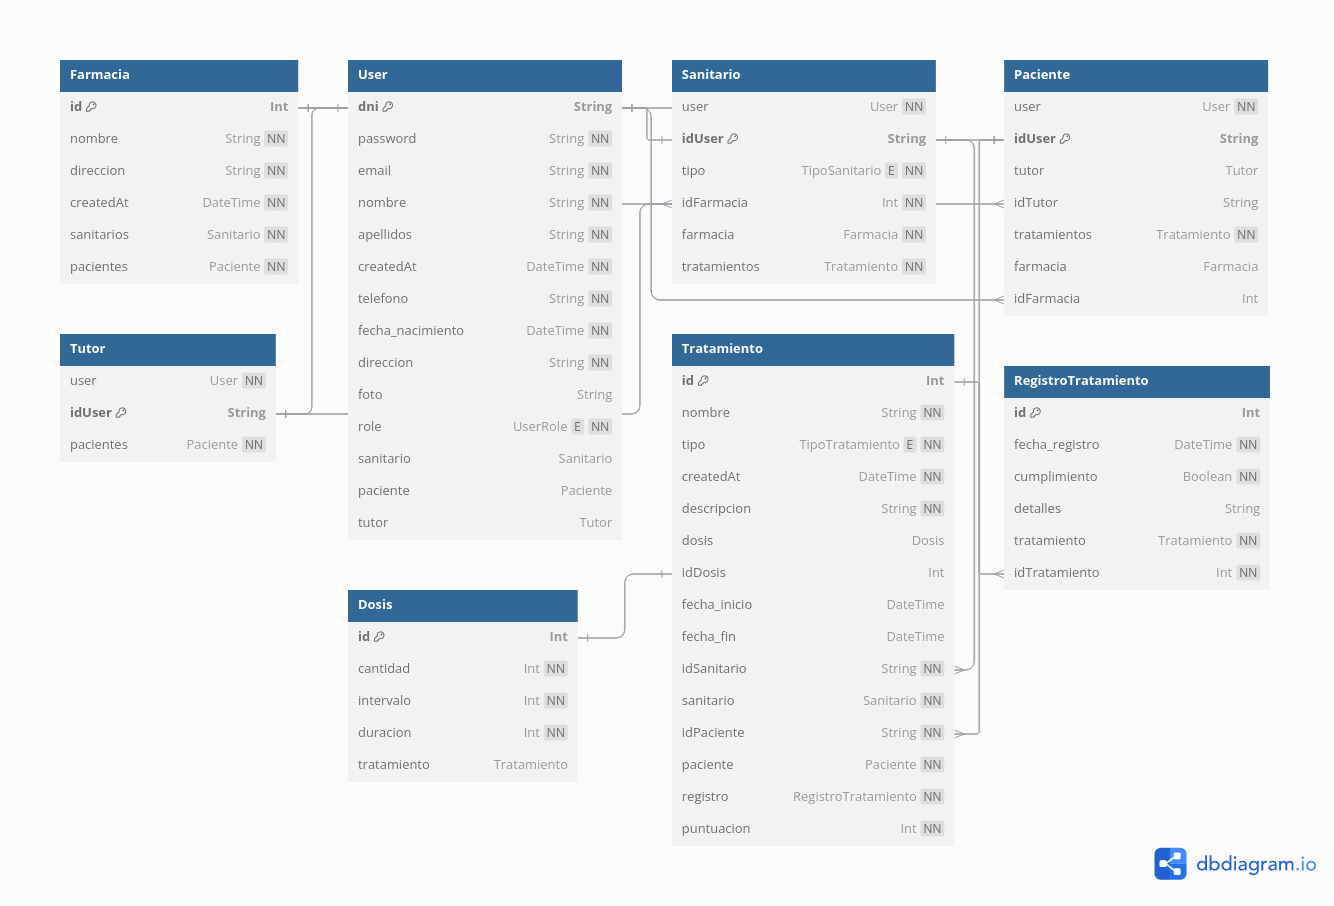
\includegraphics[width=1\textwidth]{imagenes/tablasbd.png}
	\caption{Tablas de la base de datos.}
\end{figure}

El modelo de datos establece varias relaciones clave: una farmacia puede tener múltiples sanitarios y pacientes asociados, lo que organiza a ambos grupos bajo un establecimiento específico. Cada sanitario y paciente está registrado como usuario en el sistema, permitiendo gestionar distintos roles y accesos. Los tutores pueden estar vinculados a pacientes que requieren asistencia, facilitando el seguimiento. Además, un sanitario es responsable de los tratamientos de los pacientes, cada uno de los cuales tiene su pauta de dosis y registros de adherencia, lo que permite monitorizar la evolución del tratamiento.

\subsection{Fastify, desarrollo de API}

Para configurar Fastify en este proyecto se han establecido cinco componentes principales: controladores, plugins, rutas, tests y utils. A continuación, se explica brevemente la función de cada uno y se muestra un ejemplo de código asociado.

\begin{itemize}
	\item \textbf{Controladores}. Los controladores gestionan la lógica de negocio de las operaciones solicitadas por el cliente. En este caso, el controlador maneja la creación de usuarios, validando roles y permisos de acceso según el tipo de usuario que solicita la acción.

\begin{lstlisting}[caption={Ejemplo de controlador para crear un usuario}, label={lst:createUser}]
	const createUser = async (req, reply) => {
		try {
			const { dni, email, password, nombre, apellidos, fechaNac, telefono, direccion, role, tipoSanitario, idFarmacia, foto, dniPaciente } = req.body
			const userCreator = req.user
			
			const existingUser = await prisma.user.findUnique({
				where: { dni }
			})
			
			const fechaNacimiento = new Date(fechaNac)
			if (isNaN(fechaNacimiento.getTime())) {
				return reply.status(400).send({ error: 'Fecha de nacimiento no es válida.' })
			}
			
			if (existingUser) return reply.status(400).send({ error: 'Ya existe un usuario con este DNI.' })
			
			let allowedRoles = []
			
			if (userCreator.role === ROLES.ADMIN) {
				allowedRoles = createUserPermissions[ROLES.ADMIN]
			} else if (userCreator.role === ROLES.SANITARIO) {
				if (!userCreator.sanitario) {
					userCreator.sanitario = await prisma.sanitario.findUnique({
						where: { idUser: userCreator.dni }
					})
					
					if (!userCreator.sanitario) 
					return reply.status(400).send({ error: 'El usuario sanitario no tiene información de tipo de sanitario.' })
					
				}
				allowedRoles = createUserPermissions[userCreator.sanitario.tipo] || []
				
			} else {
				return reply.status(403).send({ error: 'UNAUTHORIZED. Only an ADMIN or SANITARIO can create users.' })
			}
			
			if (!allowedRoles.includes(role)) {
				return reply.status(403).send({ error: 'UNAUTHORIZED. You are not allowed to create a user with this role.' })
			}
			
			if (role === ROLES.SANITARIO && !tipoSanitario) {
				return reply.status(400).send({ error: 'El tipo de sanitario es requerido.' })
			}
			
			if (role === ROLES.SANITARIO && !Object.values(TIPO_SANITARIO).includes(tipoSanitario)) {
				return reply.status(400).send({ error: 'El tipo de sanitario no es válido.' })
			}
			
			if (role === ROLES.SANITARIO && !idFarmacia) {
				return reply.status(400).send({ error: 'El id de la farmacia es requerido para sanitarios.' })
			}
			
			if (idFarmacia) {
				const farmacia = await prisma.farmacia.findUnique({
					where: { id: idFarmacia }
				}) 
				if (!farmacia) return reply.status(400).send({ error: 'La farmacia no existe.' })
			}
			
			if (role === ROLES.TUTOR) {
				if (!dniPaciente) {
					return reply.status(400).send({ error: 'El DNI del paciente es requerido.' })
				}
				
				const existingPatient = await prisma.paciente.findUnique({
					where: { idUser: dniPaciente }
				})
				if (!existingPatient) return reply.status(400).send({ error: 'El paciente no existe.' })
			}
			
			const hashedPassword = await hashPassword(password)
			
			const newUser = await prisma.user.create({
				data: {
					dni,
					email,
					password: hashedPassword,
					nombre,
					apellidos,
					fecha_nacimiento: fechaNacimiento,
					telefono,
					direccion,
					foto,
					role,
					sanitario: role === ROLES.SANITARIO ? {
						create: {
							tipo: tipoSanitario,
							idFarmacia
						}
					} : undefined,
					tutor: role === ROLES.TUTOR ? {
						create: {
							pacientes: { connect: { idUser: dniPaciente } } 
						}
					} : undefined,
					paciente: role === ROLES.PACIENTE ? {
						create: {
							idFarmacia
						}
					} : undefined
				}
			})
			
			if (role === ROLES.TUTOR) {
				await prisma.paciente.update({
					where: { idUser: dniPaciente }, 
					data: { idTutor: newUser.dni } 
				})
			}
			
			return reply.status(201).send({ message: 'User created successfully.', user: newUser })
			
		} catch (error) {
			console.error(error)
			reply.status(500).send({ error: 'Error creating user.' })
		}
	}
\end{lstlisting}

\newpage

\item \textbf{Plugins o \textit{Middleware}}. Los plugins extienden la funcionalidad de Fastify. En este ejemplo, se ha configurado un plugin para manejar JWT (JSON Web Tokens) y así asegurar rutas.

\begin{lstlisting}[caption={Plugin para JWT}, label={lst:pluginJWT}]
	import fp from 'fastify-plugin'
	import jwt from '@fastify/jwt'
	
	export default fp(async function (fastify, options) {
		fastify.register(jwt, {
			secret: process.env.JWT_SIGNING_SECRET
		})
		
		fastify.decorate("jwtAuth", async function (request, reply) {
			try {
				await request.jwtVerify()
			} catch (err) {
				reply.status(401).send({ err })
			}
		})
		
	})
\end{lstlisting}

\item \textbf{Rutas}. Las rutas definen los puntos de acceso a los controladores. Se utiliza preValidation con jwtAuth para proteger las rutas, asegurando que solo usuarios autenticados puedan acceder.

\begin{lstlisting}[caption={Definición de rutas para usuarios}, label={lst:userRoutes}]
	import userController from '../controllers/userController.js'
	
	async function userRouters(fastify, options) {
		fastify.post('/users/create', { preValidation: [fastify.jwtAuth] }, userController.createUser)               
		fastify.get('/users/:dni', { preValidation: [fastify.jwtAuth] }, userController.getUserByDNI)         
		fastify.get('/users', { preValidation: [fastify.jwtAuth] }, userController.getAllUsers)               
		fastify.put('/users/:dni', { preValidation: [fastify.jwtAuth] }, userController.updateUser)          
		fastify.delete('/users/:dni', { preValidation: [fastify.jwtAuth] }, userController.deleteUser)        
		fastify.get('/users/sanitarios/:dni', { preValidation: [fastify.jwtAuth] }, userController.getSanitarioData) 
		fastify.get('/users/pacientes/:dni', { preValidation: [fastify.jwtAuth] }, userController.getPacienteData)   
		fastify.get('/users/tutores/:dni', { preValidation: [fastify.jwtAuth] }, userController.getTutorData)  
		fastify.get('/users/pacientes/sinfarmacia', { preValidation: [fastify.jwtAuth] }, userController.getPacientesSinFarmacia)
		fastify.put('/users/:dni/password', { preValidation: [fastify.jwtAuth] }, userController.updatePassword)
	}
	
	export default userRouters
\end{lstlisting}
\newpage

\item \textbf{Tests}. Los tests validan la funcionalidad del sistema, asegurando que las operaciones cumplen con las expectativas. En este ejemplo, se verifica que un farmacéutico pueda crear un tratamiento farmacológico para un paciente.

\begin{lstlisting}[caption={Ejemplo de test para creación de tratamiento}, label={lst:createTreatmentTest}]
	it('Debería permitir al farmacéutico crear un tratamiento farmacológico para un paciente', async () => {
		const farmaceuticoLogin = await fastify.inject({
			method: 'POST',
			url: '/api/login',
			payload: { dni: '33445566G', password: 'farmaceutico567' }
		})
		expect(farmaceuticoLogin.statusCode).to.equal(200)
		const farmaceuticoToken = JSON.parse(farmaceuticoLogin.payload).token
		
		const tratamientoFarmacologicoResponse = await fastify.inject({
			method: 'POST',
			url: '/api/tratamientos/create',
			headers: { Authorization: `Bearer ${farmaceuticoToken}` },
			payload: {
				nombre: 'Tratamiento Antibiotico',
				tipo: 'FARMACOLOGICO',
				descripcion: 'Tratamiento para infección',
				idPaciente: pacienteId1,
				dosis: {
					cantidad: 500,
					intervalo: 8,
					duracion: 10
				}
			}
		})
		expect(tratamientoFarmacologicoResponse.statusCode).to.equal(201)
		const tratamiento = JSON.parse(tratamientoFarmacologicoResponse.payload)
		tratamientoId1 = tratamiento.id
	})
\end{lstlisting}


\item \textbf{Utils}. Los utils agrupan funciones de utilidad que se utilizan en distintos puntos del código. En este caso, se incluyen funciones para encriptar y comparar contraseñas.
\begin{lstlisting}[caption={Funciones de utilidad para contraseñas}, label={lst:utilsPassword}]
	import bcrypt from 'bcrypt';
	
	const SALT_ROUNDS = 12
	
	export async function hashPassword(password) {
		try {
			return await bcrypt.hash(password, SALT_ROUNDS)
		} catch (error) {
			console.error('Error hashing password:', error)
			throw new Error('Failed to hash password')
		}
	}
	
	export const comparePassword = async (password, hashedPassword) => {
		return bcrypt.compare(password, hashedPassword)
	}
\end{lstlisting}


\item \textbf{Configuración del servidor}. En el archivo \texttt{server.js} se configura el servidor Fastify, que actúa como el núcleo de la aplicación, integrando diferentes funcionalidades a través de plugins, rutas y configuraciones específicas. \\

En \texttt{server.js} primero se importa y configura Fastify, iniciando el servidor con un logger detallado para rastrear eventos y errores. Luego, se registra el plugin cors, permitiendo el acceso desde distintas fuentes con los métodos HTTP especificados. También se habilita el plugin JWT para manejar la autenticación con tokens, asegurando que solo los usuarios autorizados puedan acceder a ciertas rutas.

A continuación, se registra un parser para solicitudes en formato JSON. Después se configuran las rutas principales del servidor (farmaciaRoutes, userRoutes, tratamientoRoutes y authRoutes), todas accesibles bajo el prefijo /api. Finalmente, se define una ruta por defecto para probar el funcionamiento del servidor y se implementa una función para iniciar el servidor en el puerto indicado, gestionando cualquier error que ocurra al iniciar.

\begin{lstlisting}[caption={Archivo server.js - Configuración del servidor Fastify}, label={lst:server-js}]
	import Fastify from 'fastify'
	import { PORT } from './config/init.js'
	import cors from '@fastify/cors'; 
	import farmaciaRoutes from './routes/farmaciaRoutes.js'
	import userRoutes from './routes/userRoutes.js'
	import tratamientoRoutes from './routes/tratamientoRoutes.js'
	import authRoutes from './routes/authRoutes.js'
	import jwtPlugin from './plugins/jwtPlugin.js'
	
	const fastify = Fastify({
		logger: {
			level: 'trace',
			transport: {
				target: 'pino-pretty',
			}
		}
	})
	

	fastify.register(cors, { 
		origin: true, 
		methods: ['POST', 'GET', 'PUT', 'DELETE', 'OPTIONS'],
	})
	
	fastify.register(jwtPlugin)
	
	// Parser para contenido JSON
	fastify.addContentTypeParser('application/json', { parseAs: 'string' }, fastify.getDefaultJsonParser('strict'))
	
	fastify.register(farmaciaRoutes, { prefix: '/api' })
	fastify.register(userRoutes, { prefix: '/api' })
	fastify.register(tratamientoRoutes, { prefix: '/api' })
	fastify.register(authRoutes, { prefix: '/api' })
	
	// Ruta por defecto
	fastify.get('/', async function handler (request, reply) {
		return { hello: 'world' }
	})
	
	const startServer = async () => {
		try {
			await fastify.listen({ port: PORT })
			console.log(`Server is running on port ${ PORT }`)
			
		} catch (err) {
			fastify.log.error(err)
			process.exit(1)
		}
	}
	
	export default fastify
	startServer()
\end{lstlisting}


\end{itemize}

\subsection{Dependencias de Node.js}
 Las dependencias son módulos externos que un proyecto necesita para funcionar correctamente. Estas se especifican en el archivo \texttt{package.json} bajo las secciones \texttt{dependencies} y \texttt{devDependencies}.
\begin{itemize} 
	\item \textbf{@fastify/cors}: Permite configurar CORS (Cross-Origin Resource Sharing) en Fastify, lo que habilita solicitudes desde distintos dominios y métodos HTTP específicos. 
	\item \textbf{@fastify/jwt}: Gestiona la autenticación mediante JSON Web Tokens (JWT), proporcionando seguridad al sistema al verificar usuarios. 
	\item \textbf{@prisma/client}: Cliente de Prisma para interactuar con la base de datos para realizar consultas y operaciones sobre el esquema definido en \texttt{schema.prisma}. 
	\item \textbf{bcrypt}: Utilizado para encriptar contraseñas.
	\item \textbf{fastify-plugin}: Facilita la creación y uso de plugins en Fastify. 
	\item \textbf{pino-pretty}: Formatea los logs generados por Fastify para hacerlos más legibles durante el desarrollo. 
	\item \textbf{chai}: Biblioteca de aserciones para escribir pruebas, proporcionando múltiples estilos de aserción para verificar resultados. 
	\item \textbf{mocha}: Marco de pruebas que permite ejecutar y estructurar pruebas, facilitando la verificación de la funcionalidad del sistema.  
	\item \textbf{prisma-dbml-generator}: Genera diagramas de entidad-relación (ERD) en formato DBML, visualizando el modelo de datos definido en Prisma.
\end{itemize}

\subsection{Flujo de peticiones a API} El flujo de una petición a la API en Fastify comienza cuando un cliente envía una solicitud a una ruta específica, como POST \texttt{/api/users/create}. Primero, la ruta definida en el archivo de rutas (por ejemplo, userRoutes.js) intercepta la solicitud. Si la ruta está protegida, se aplica una pre-validación, utilizando el plugin de autenticación JWT (como jwtPlugin.js), que verifica que el cliente esté autenticado. Una vez autenticado, el controlador correspondiente (en este caso, createUser en userController.js) se encarga de procesar la lógica principal de la solicitud, como validar datos y realizar operaciones en la base de datos usando Prisma. Finalmente, la respuesta se envía al cliente, indicando el éxito o el error de la operación. Este flujo asegura un manejo estructurado y seguro de las solicitudes en la API.

\newpage

\subsection{Organización de directorios} Finalmente, la estructura de directorios para el backend se muestra como sigue:
\begin{figure}[h!]
	\centering
	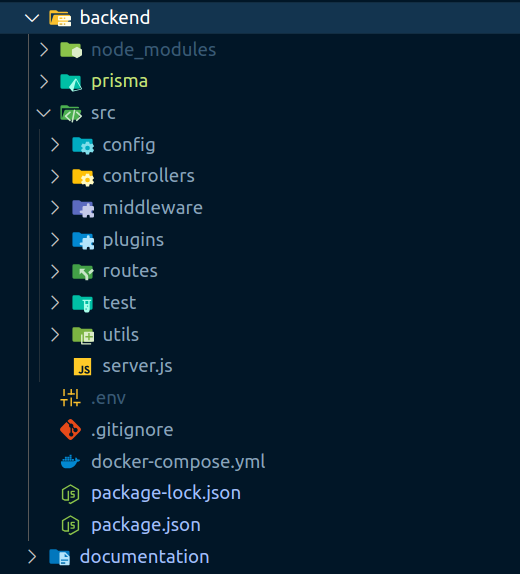
\includegraphics[width=0.5\textwidth]{imagenes/orgback.png}
	\caption{Directorios del backend.}
\end{figure}



\section{Desarrollo del frontend}

\subsection{Desarrollo del frontend con Astro}

En el desarrollo del frontend se ha utilizado Astro y se ha configurado para que tenga un layout base que permita establecer una estructura y diseño consistentes en todas las páginas de la aplicación. Este layout se configura en el archivo \texttt{Layout.astro} y contiene componentes comunes como la barra de navegación, pie de página y verificación de autenticación.

\subsubsection{Configuración del layout base}

El layout base incluye los componentes esenciales y define cuándo deben mostrarse, basándose en la ruta actual. A continuación se presenta el código del archivo \texttt{Layout.astro}:

\begin{lstlisting}[language=html, caption={Layout base en Astro}]
	---
	import Navbarreact from "../components/ui/Navbar";
	import Footer from "../components/ui/footer.astro";
	import AuthCheck from "../components/sections/checks/AuthCheck";
	
	interface Props {
		title: string;
	}
	
	const { title } = Astro.props;
	const currentPath = Astro.url.pathname;
	const showNavbar = currentPath !== "/" && currentPath !== "/login";
	const showLimit = showNavbar;
	const authCheck = showNavbar;
	---
	
	<!doctype html>
	<html lang="es" class="lenis lenis-smooth scroll-pt-5">
	<head>
	<meta charset="UTF-8" />
	<meta name="description" content="Astro description" />
	<meta name="viewport" content="width=device-width" />
	<link rel="icon" type="image/svg+xml" href="/favicon.svg" />
	<meta name="author" content="VIDICAN, MIHNEA IOAN" />
	<meta name="generator" content={Astro.generator} />
	<title>{title}</title>
	</head>
	<style>
	html {
		overflow-y: scroll;
	}
	</style>
	<body class="bg-base-100 w-full">
	<div class="grid min-h-screen grid-rows-[auto_1fr_auto]">
	{showNavbar && <Navbarreact client:load />}
	{authCheck && <AuthCheck client:load/>}
	
	<main>
	<div class={showLimit ? "max-w-screen-xl mx-auto" : ""}>
	<slot />
	</div>
	</main>
	
	<Footer />
	</div>
	</body>
	<script>
	import "../../assets/scripts/lenisSmoothScroll.js";
	</script>
	</html>
\end{lstlisting}

En este layout, se configuran los componentes comunes \texttt{Navbarreact}, \texttt{Footer}, y \texttt{AuthCheck}, que se muestran solo en determinadas rutas. La etiqueta \texttt{<slot />} permite incluir el contenido de cada vista específica dentro de esta estructura.

\subsubsection{Uso del layout en una vista específica}

Para cada página, se utiliza el layout importándolo y envolviendo el contenido dentro de él. A continuación, se muestra cómo se utiliza el layout en la página de inicio de sesión, \texttt{login.astro}:

\begin{lstlisting}[language=html, caption={Uso del Layout en login.astro}]
	---
	import Layout from "../layouts/Layout.astro";
	import LoginForm from "../components/sections/LoginForm.jsx";
	---
	
	<Layout title="Inicio de sesión">
	<LoginForm client:load />
	</Layout>
\end{lstlisting}

\begin{itemize}
	\item Aquí, el componente \texttt{LoginForm} se incluye dentro del layout, configurando así la página de inicio de sesión con el mismo estilo y estructura que el layout base.
	\item Esto permite mantener una estructura común en toda la aplicación.
\end{itemize}

\subsection{Uso de React}

Para añadir interactividad en el frontend, como se ha mencionado previamente, se ha utilizado \textbf{React}. A continuación se muestra un ejemplo del archivo \texttt{TratamientosForm.jsx}, un componente que permite a un sanitario, bien sea un farmacéutico o técnico de farmacia, crear un tratamiento específico para un paciente. Este formulario incluye validación de datos y mensajes de éxito o error según el resultado de la petición.

\begin{lstlisting}[caption={TratamientoForm.jsx - Formulario de creación de tratamiento para un paciente}]
	import { useState, useEffect } from "react";
	import SanitarioCheck from "../checks/SanitarioCheck";
	
	const TratamientoForm = () => {
		const [nombre, setNombre] = useState("");
		const [descripcion, setDescripcion] = useState("");
		const [tipo, setTipo] = useState("");
		const [dosis, setDosis] = useState({ cantidad: "", intervalo: "", duracion: "" });
		const [fechaFin, setFechaFin] = useState("");
		const [idFarmacia, setIdFarmacia] = useState(null);
		const [pacientes, setPacientes] = useState([]);
		const [idPaciente, setIdPaciente] = useState("");
		const [isLoading, setIsLoading] = useState(false);
		const [errorMessage, setErrorMessage] = useState("");
		const [successMessage, setSuccessMessage] = useState("");
		
		useEffect(() => {
			const fetchSanitarioData = async () => {
				const user = JSON.parse(sessionStorage.getItem("user"));
				if (user && user.dni) {
					try {
						const token = sessionStorage.getItem("jwtToken");
						const response = await fetch(`http://localhost:3000/api/users/sanitarios/${user.dni}`, {
							headers: { Authorization: `Bearer ${token}` },
						});
						const data = await response.json();
						if (response.ok) {
							setIdFarmacia(data.idFarmacia);
							fetchPacientes(data.idFarmacia, token);
						} else {
							setErrorMessage(data.error || "No se pudo obtener el ID de la farmacia.");
						}
					} catch (error) {
						console.error("Error al obtener los datos del sanitario:", error);
						setErrorMessage("Error de conexión al obtener los datos del sanitario.");
					}
				} else {
					setErrorMessage("No se pudo obtener el DNI del usuario logeado.");
				}
			};
			
			fetchSanitarioData();
		}, []);
		
		const fetchPacientes = async (farmaciaId, token) => {
			try {
				const response = await fetch(`http://localhost:3000/api/farmacias/${farmaciaId}/pacientes`, {
					method: "GET",
					headers: { Authorization: `Bearer ${token}` },
				});
				const data = await response.json();
				if (response.ok) {
					setPacientes(data);
				} else {
					setErrorMessage(data.error || "Error al obtener los pacientes.");
				}
			} catch (error) {
				console.error("Error fetching pacientes:", error);
				setErrorMessage("Hubo un problema con la conexión. Inténtelo de nuevo más tarde.");
			}
		};
		
		const validateForm = () => {
			if (!nombre || !descripcion || !tipo || !idPaciente) {
				setErrorMessage("Todos los campos son obligatorios.");
				return false;
			}
			if (tipo === "FARMACOLOGICO" && (!dosis.cantidad || !dosis.intervalo || !dosis.duracion)) {
				setErrorMessage("Todos los campos de dosis son obligatorios para un tratamiento farmacológico.");
				return false;
			}
			if (tipo === "NO_FARMACOLOGICO" && !fechaFin) {
				setErrorMessage("La fecha de fin es obligatoria para un tratamiento no farmacológico.");
				return false;
			}
			setErrorMessage("");
			return true;
		};
		
		const handleSubmit = async (e) => {
			e.preventDefault();
			if (!validateForm()) return;
			
			setIsLoading(true);
			setErrorMessage("");
			setSuccessMessage("");
			
			const data = {
				nombre,
				descripcion,
				tipo,
				idPaciente,
				dosis: tipo === "FARMACOLOGICO" ? dosis : null,
				fecha_fin: tipo === "NO_FARMACOLOGICO" ? fechaFin : null,
			};
			
			try {
				const response = await fetch("http://localhost:3000/api/tratamientos/create", {
					method: "POST",
					headers: {
						"Content-Type": "application/json",
						Authorization: `Bearer ${sessionStorage.getItem("jwtToken")}`,
					},
					body: JSON.stringify(data),
				});
				
				const responseData = await response.json();
				if (response.ok) {
					setSuccessMessage("Tratamiento creado con éxito");
					setTimeout(() => setSuccessMessage(""), 3000);
					setNombre("");
					setDescripcion("");
					setTipo("");
					setDosis({ cantidad: "", intervalo: "", duracion: "" });
					setFechaFin("");
					setIdPaciente("");
				} else {
					setErrorMessage(responseData.error || "Error al crear el tratamiento");
				}
			} catch (error) {
				console.error("Hubo un error de conexión:", error);
				setErrorMessage("Hubo un problema con la conexión. Inténtelo de nuevo más tarde.");
			} finally {
				setIsLoading(false);
			}
		};
		
		return (
		<SanitarioCheck>
		<div className="flex justify-center text-center m-10">
		<div className="breadcrumbs text-xl">
		<ul>
		<li><a href="/dashboard">Panel de control</a></li>
		<li><a href="/tratamientos">Tratamientos</a></li>
		<li>Crear tratamiento a paciente</li>
		</ul>
		</div>
		</div>
		
		<div className="flex items-center justify-center m-10">
		<div className="card bg-base-100 w-full max-w-xl shadow-2xl p-8">
		<form onSubmit={handleSubmit}>
		</form>
		</div>
		</div>
		</SanitarioCheck>
		);
	};
	
	export default TratamientoForm;
\end{lstlisting}

\newpage
\subsection{Uso de Tailwind CSS y DaisyUI}

Para la gestión de estilos en el frontend se ha optado por \textbf{Tailwind CSS}, un framework CSS que permite aplicar estilos mediante clases predefinidas. Además, se ha integrado la librería \textbf{DaisyUI} sobre Tailwind CSS, la cual proporciona componentes predefinidos y personalizables, como botones, tarjetas, formularios, entre otros. 

A continuación se presenta un ejemplo de cómo se usa DaisyUI para el componente de tarjeta en el formulario de tratamiento:

\begin{lstlisting}[language=html, caption={Ejemplo de componente de tarjeta con DaisyUI}]
	<div className="card bg-base-100 w-full max-w-xl shadow-2xl p-8">
	<form onSubmit={handleSubmit}>
	<div className="form-control mb-4">
	<input
	type="text"
	className="input input-bordered input-primary"
	placeholder="Nombre del tratamiento"
	value={nombre}
	onChange={(e) => setNombre(e.target.value)}
	required
	/>
	</div>
	
	<div className="form-control mb-4">
	<textarea
	className="textarea textarea-primary"
	placeholder="Descripción"
	value={descripcion}
	onChange={(e) => setDescripcion(e.target.value)}
	required
	></textarea>
	</div>
	
	<div className="form-control mt-4">
	<button className="btn btn-primary text-white" disabled={isLoading}>
	{isLoading ? (
		<span className="loading loading-dots loading-lg text-white"></span>
		) : (
		"Crear tratamiento"
		)}
	</button>
	</div>
	</form>
	</div>
\end{lstlisting}

\subsection{Dependencias adicionales en el Frontend}

Para el desarrollo del frontend, además de \textbf{Astro} y \textbf{DaisyUI}, se han integrado otras dependencias que complementan la funcionalidad y estilización de la aplicación. A continuación se detallan:

\begin{itemize}
	\item \textbf{lenis}: Esta biblioteca permite suavizar el desplazamiento dentro de la aplicación, proporcionando una experiencia de usuario fluida al navegar entre secciones.
	
	\item \textbf{react-dom}: texttt{react-dom} Facilita el renderizado de los componentes interactivos de React en el DOM.
	
	\item \textbf{react-router-dom}: Esta biblioteca gestiona el enrutamiento de la aplicación para permitir la navegación entre diferentes vistas.
	
\end{itemize}

\subsection{Organización de directorios} Finalmente, la estructura de directorios para el frontend se muestra como sigue:
\begin{figure}[h!]
	\centering
	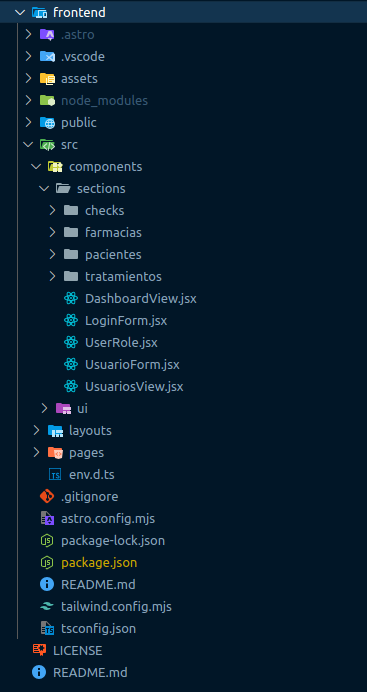
\includegraphics[width=0.5\textwidth]{imagenes/orgfront.png}
	\caption{Directorios del frontend.}
\end{figure}

\newpage
\section{Diseño de la interfaz de usuario}.
La interfaz de usuario se ha visto inspirada en el aspecto visual de un proyecto de código abierto, ScrewFast \cite{screwfast}, el cual combina el uso de Astro y Tailwind CSS para proporcionar una página web rápida y atractiva. \\

Para PharmAD predomina los colores verde, en diferentes tonalidades, y blanco. Se muestran imágenes acerca de las diferentes secciones de la plataforma.


\begin{figure}[h!]
	\centering
	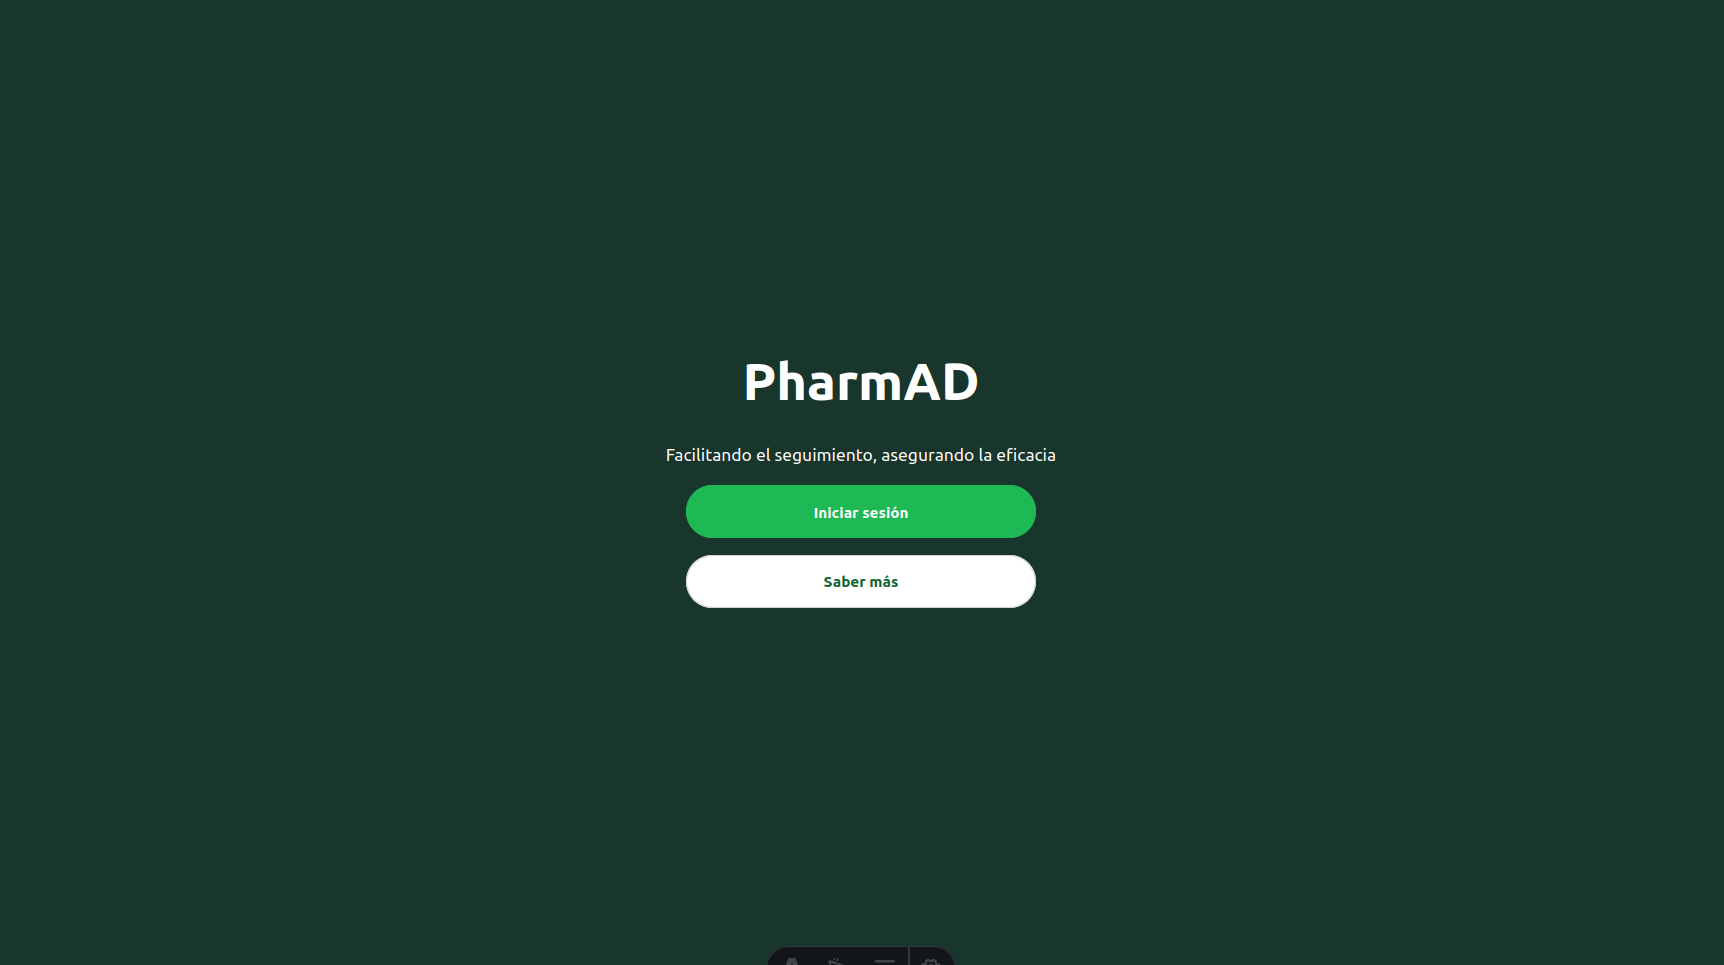
\includegraphics[width=0.9\textwidth]{imagenes/landing.png}
	\caption{Landing page.}
\end{figure}

\begin{figure}[h!]
	\centering
	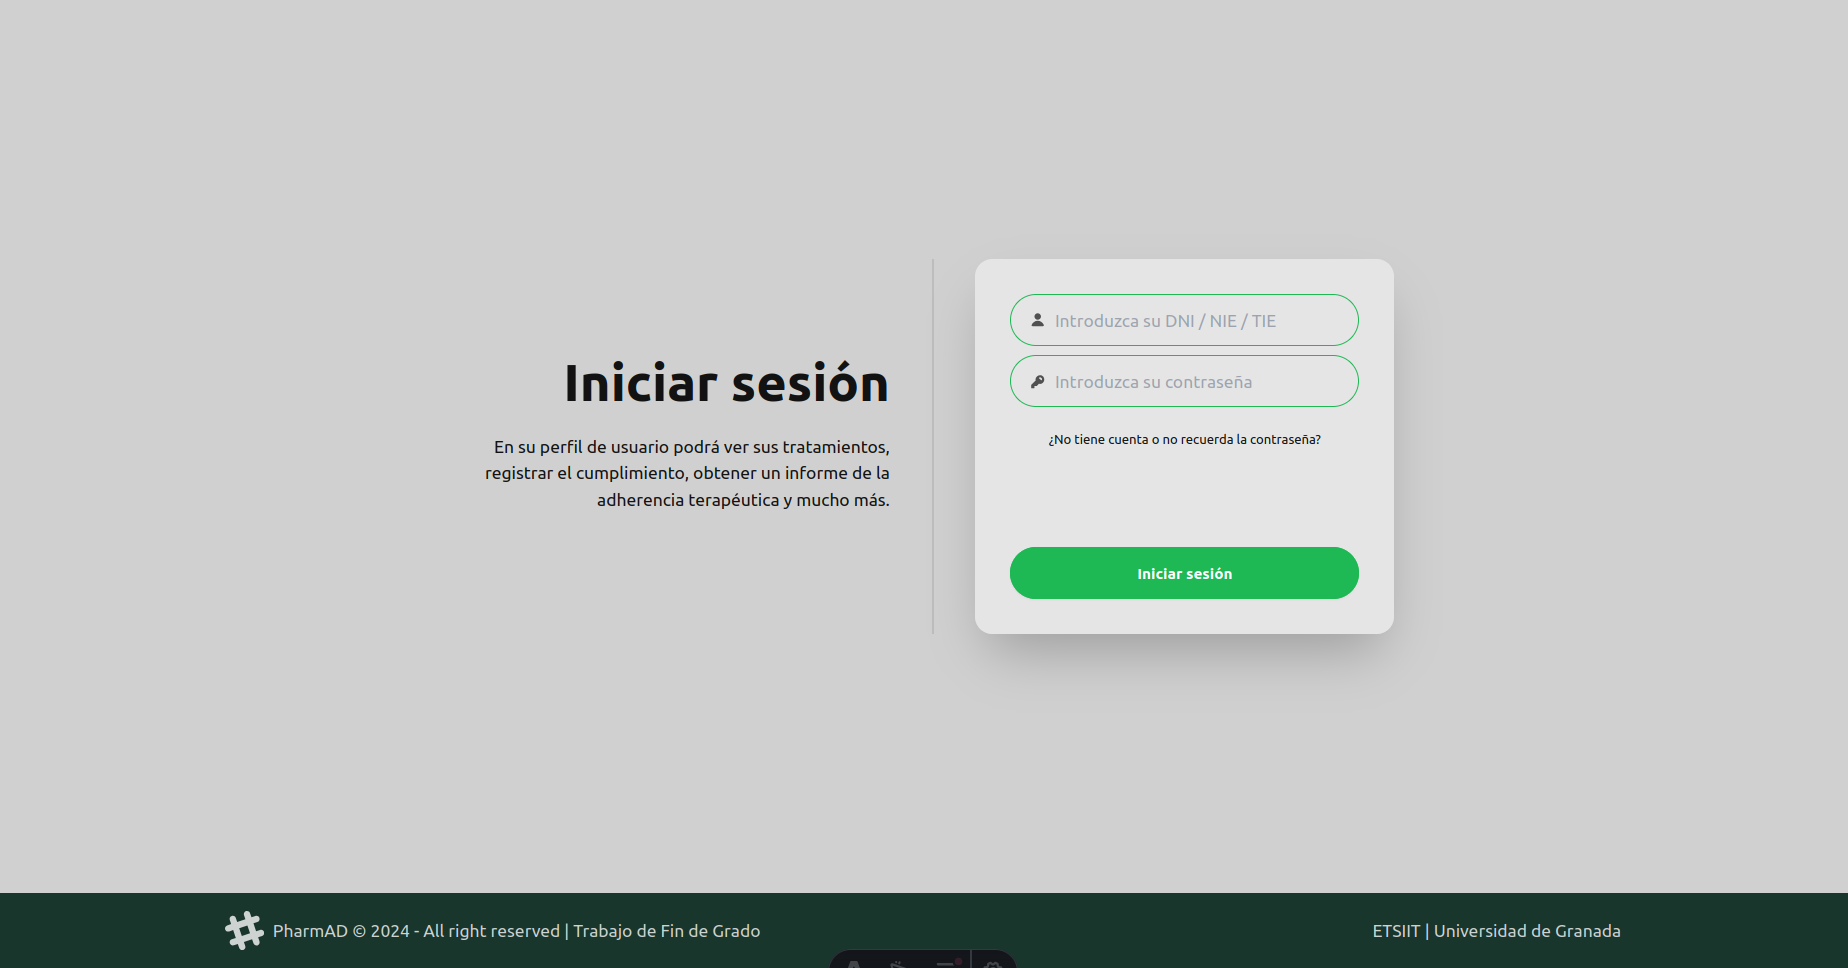
\includegraphics[width=0.9\textwidth]{imagenes/login.png}
	\caption{Pantalla de inicio de sesión.}
\end{figure}


\begin{figure}[h!]
	\centering
	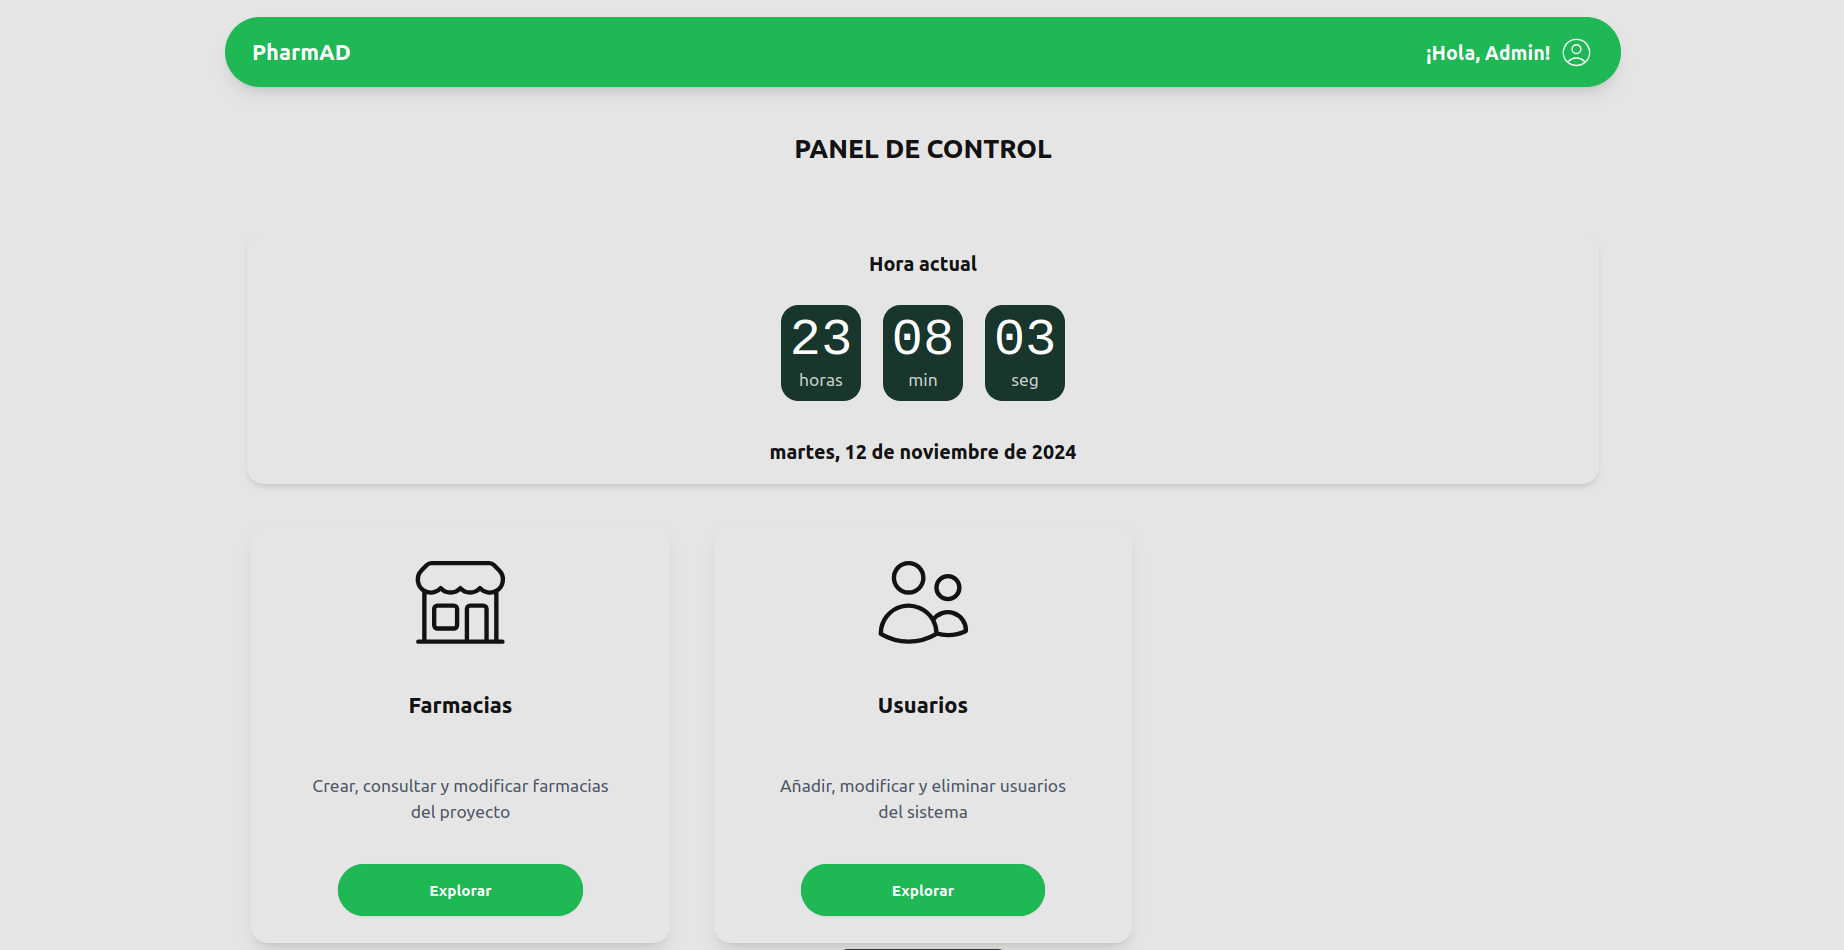
\includegraphics[width=0.9\textwidth]{imagenes/admin.png}
	\caption{Panel de control del administrador.}
\end{figure}


\begin{figure}[h!]
	\centering
	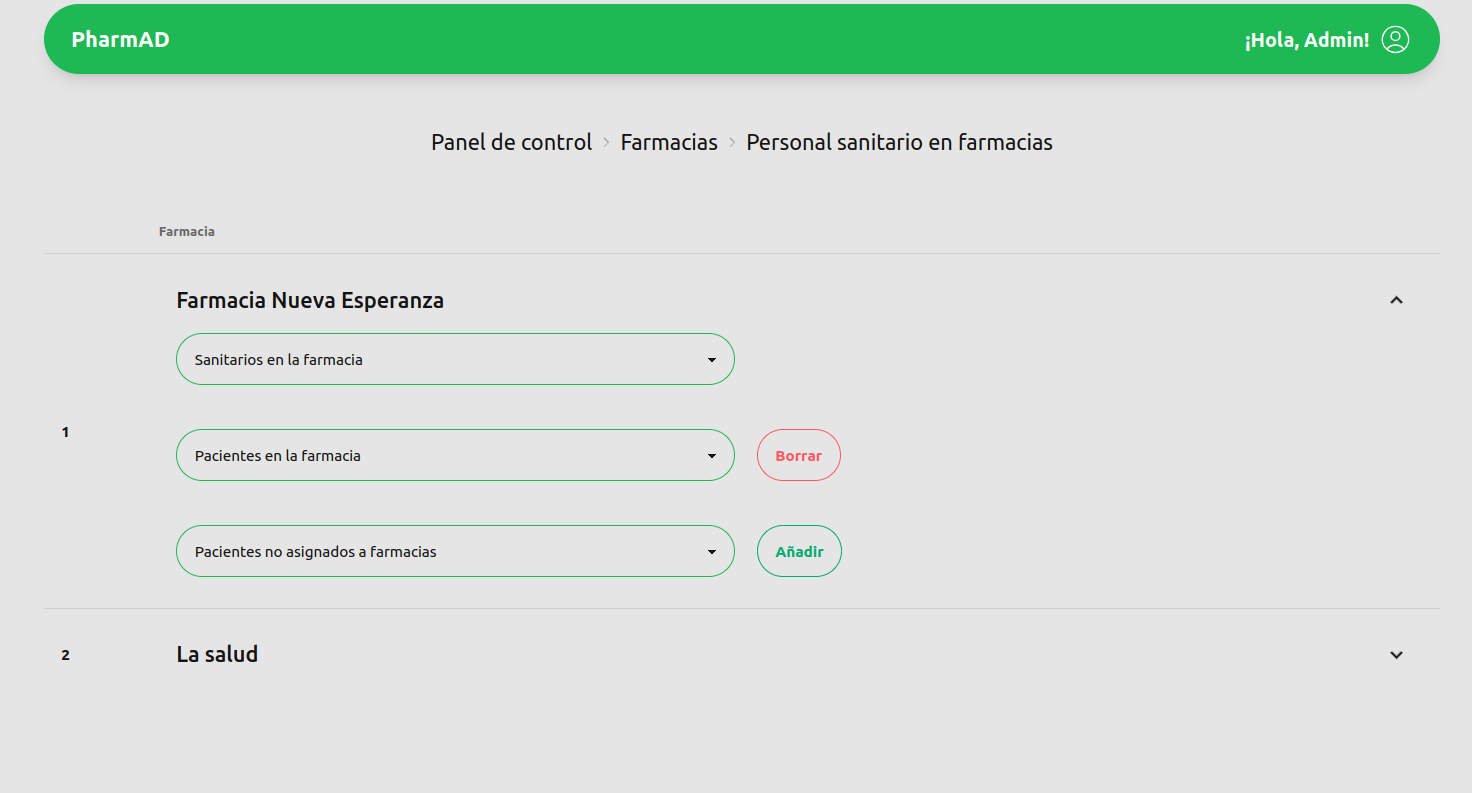
\includegraphics[width=0.9\textwidth]{imagenes/personalfarmacias.png}
	\caption{Lista de personal de farmacias para el administrador.}
\end{figure}


\begin{figure}[h!]
	\centering
	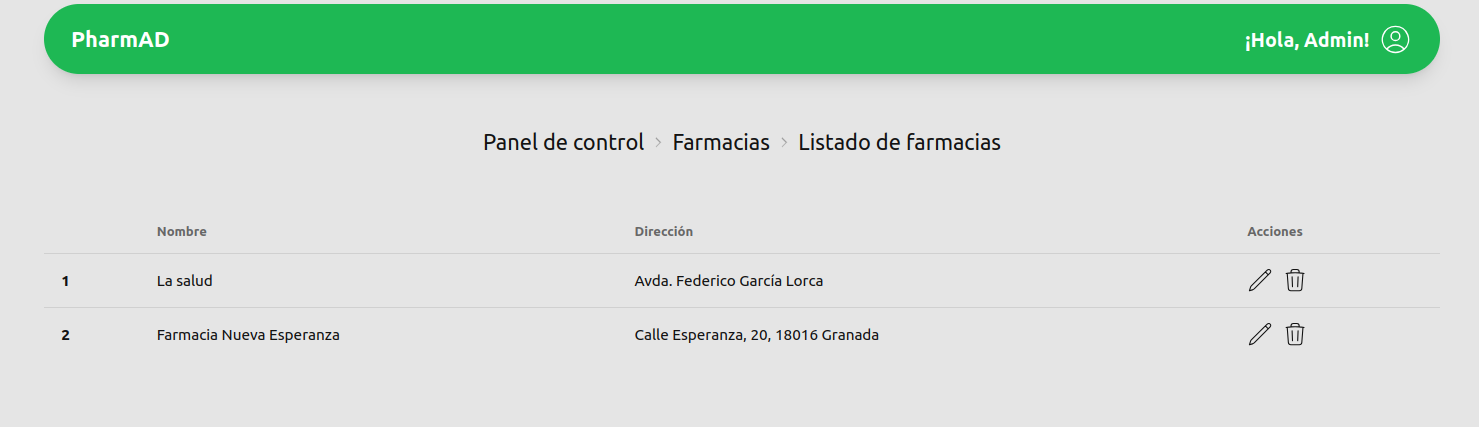
\includegraphics[width=0.9\textwidth]{imagenes/listafarmacias.png}
	\caption{Listado de farmacias para el administrador}
\end{figure}

\begin{figure}[h!]
	\centering
	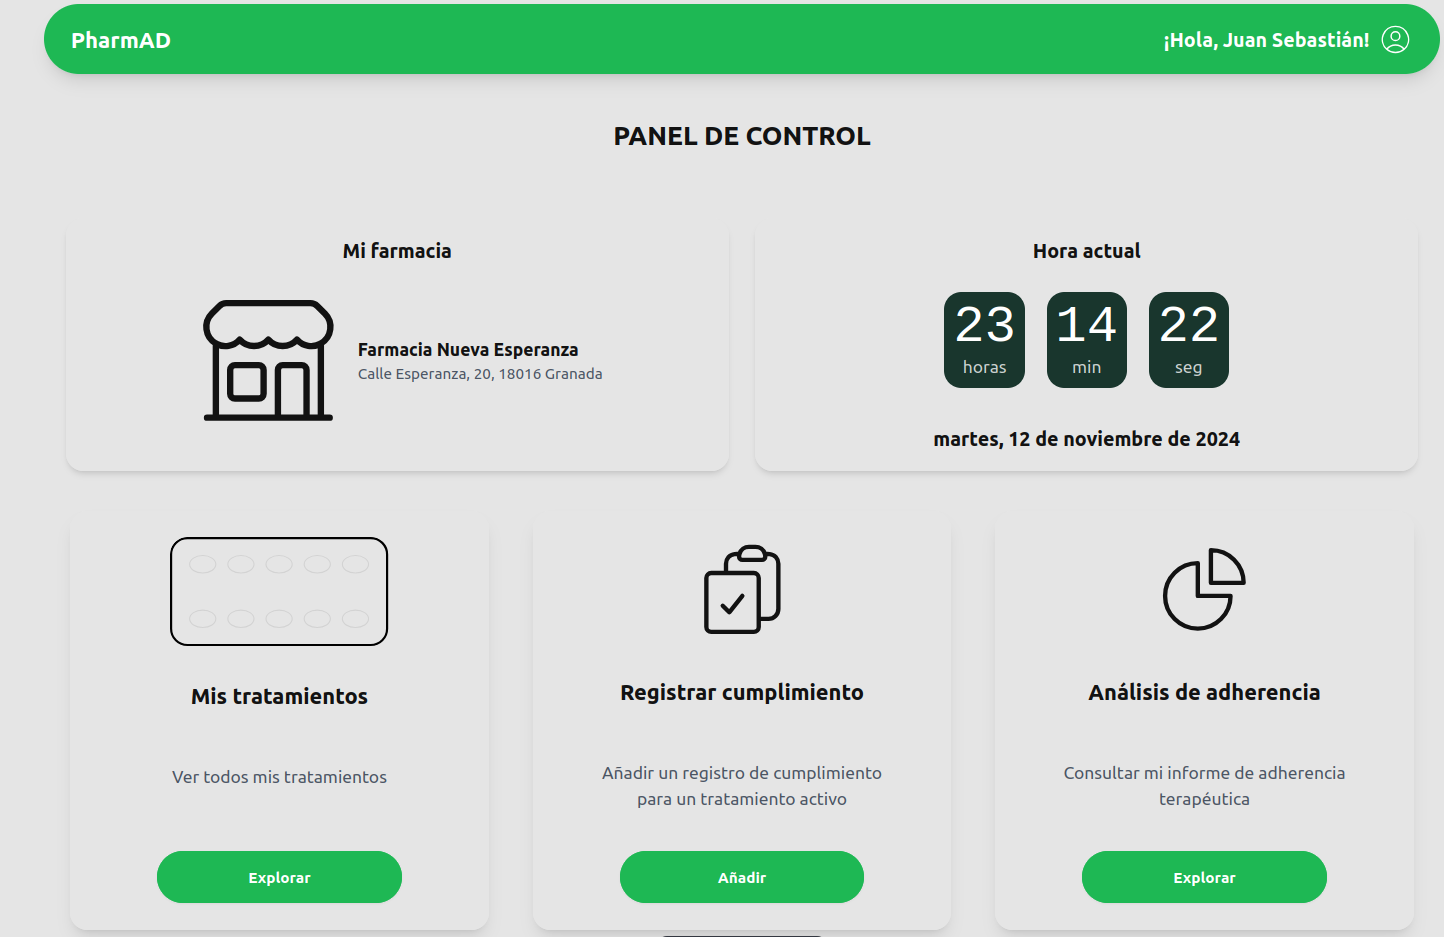
\includegraphics[width=0.9\textwidth]{imagenes/user.png}
	\caption{Panel de control del usuario.}
\end{figure}


\begin{figure}[h!]
	\centering
	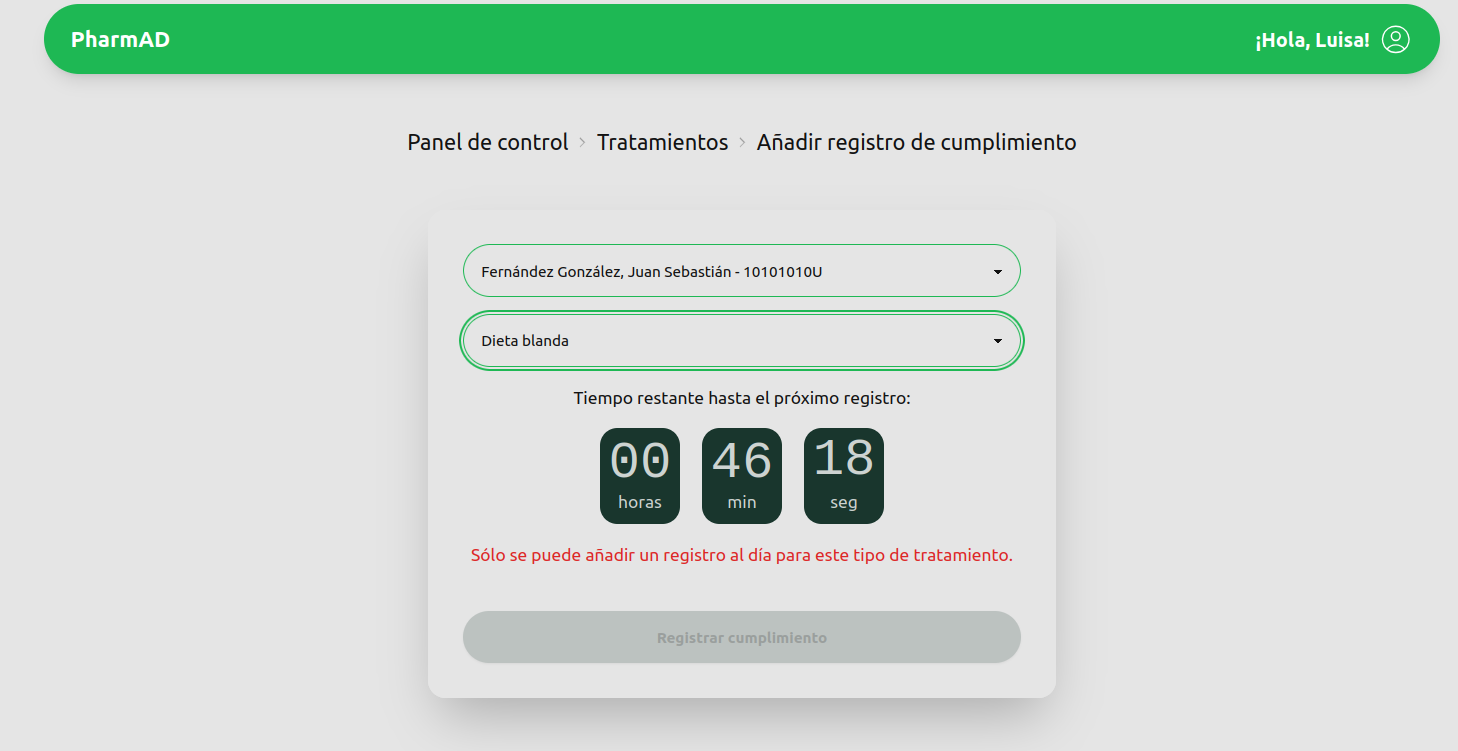
\includegraphics[width=0.9\textwidth]{imagenes/registro.png}
	\caption{Vista de registro de cumplimiento para el usuario.}
\end{figure}

\begin{figure}[h!]
	\centering
	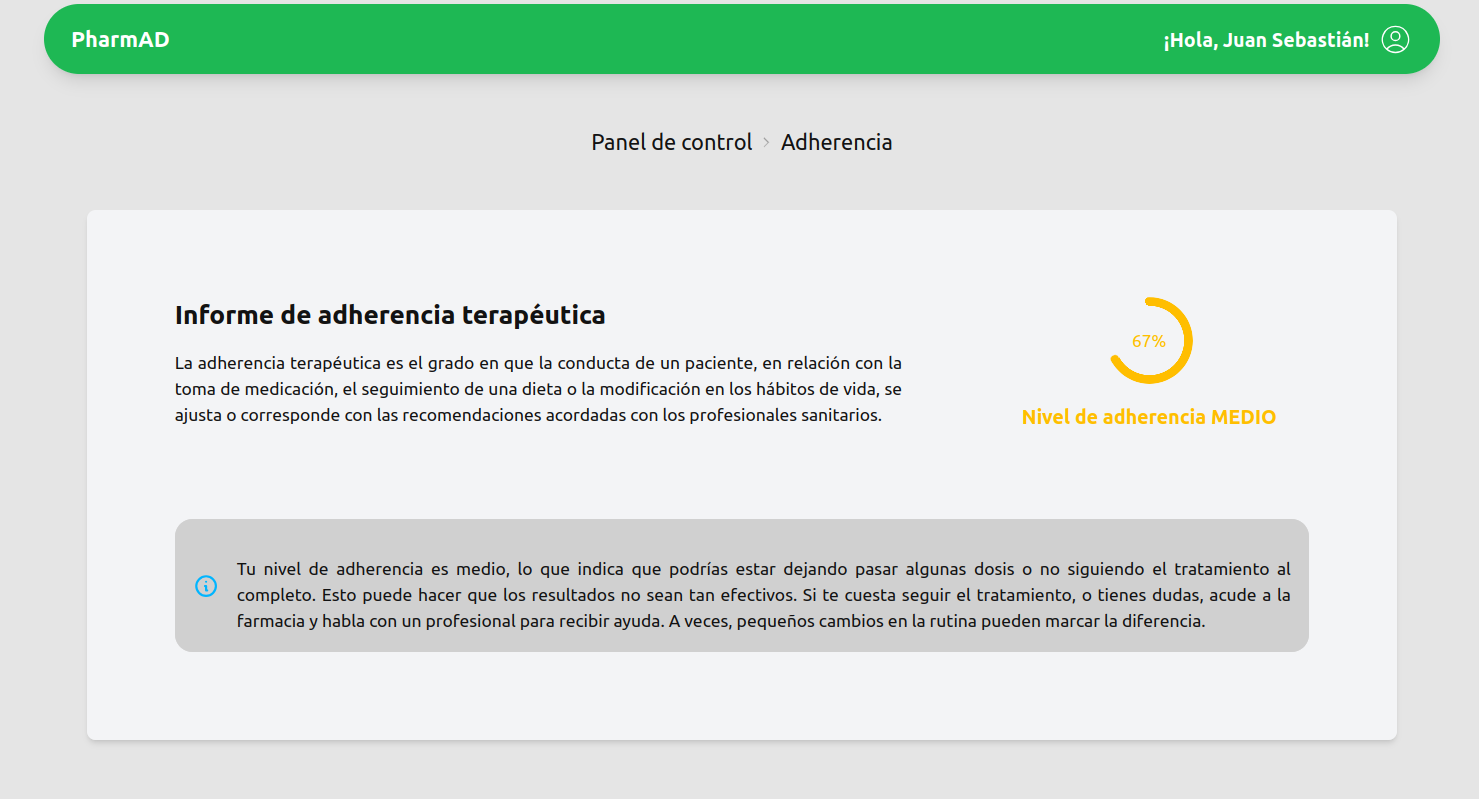
\includegraphics[width=0.9\textwidth]{imagenes/adherencia.png}
	\caption{Vista del informe de adherencia terapéutica para el usuario.}
\end{figure}


\begin{figure}[h!]
	\centering
	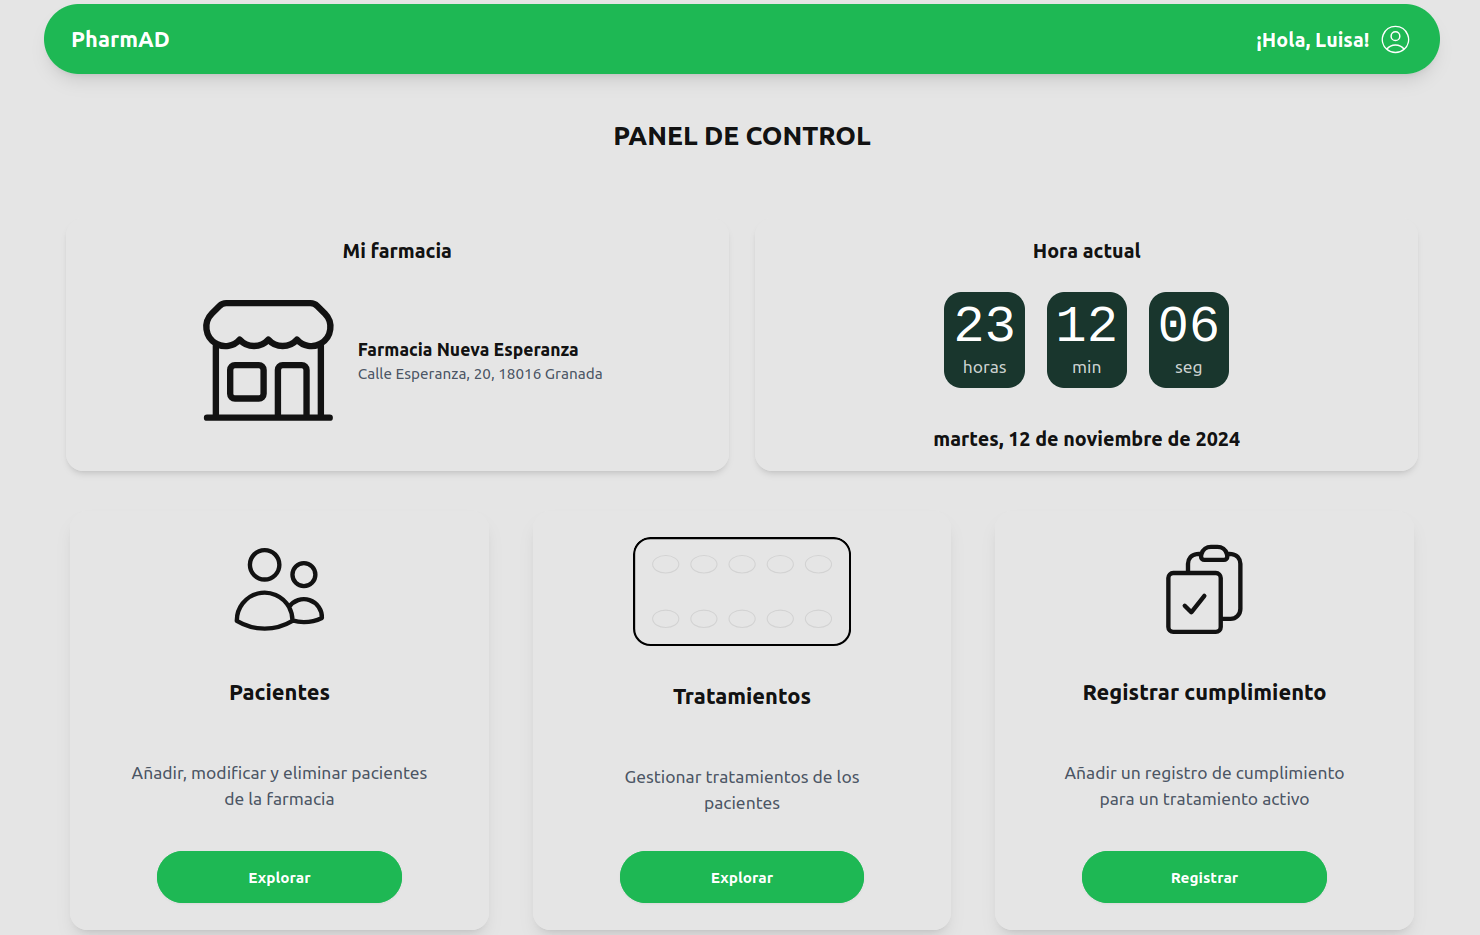
\includegraphics[width=0.9\textwidth]{imagenes/farmaceutico.png}
	\caption{Panel de control para el farmacéutico.}
\end{figure}

\begin{figure}[h!]
	\centering
	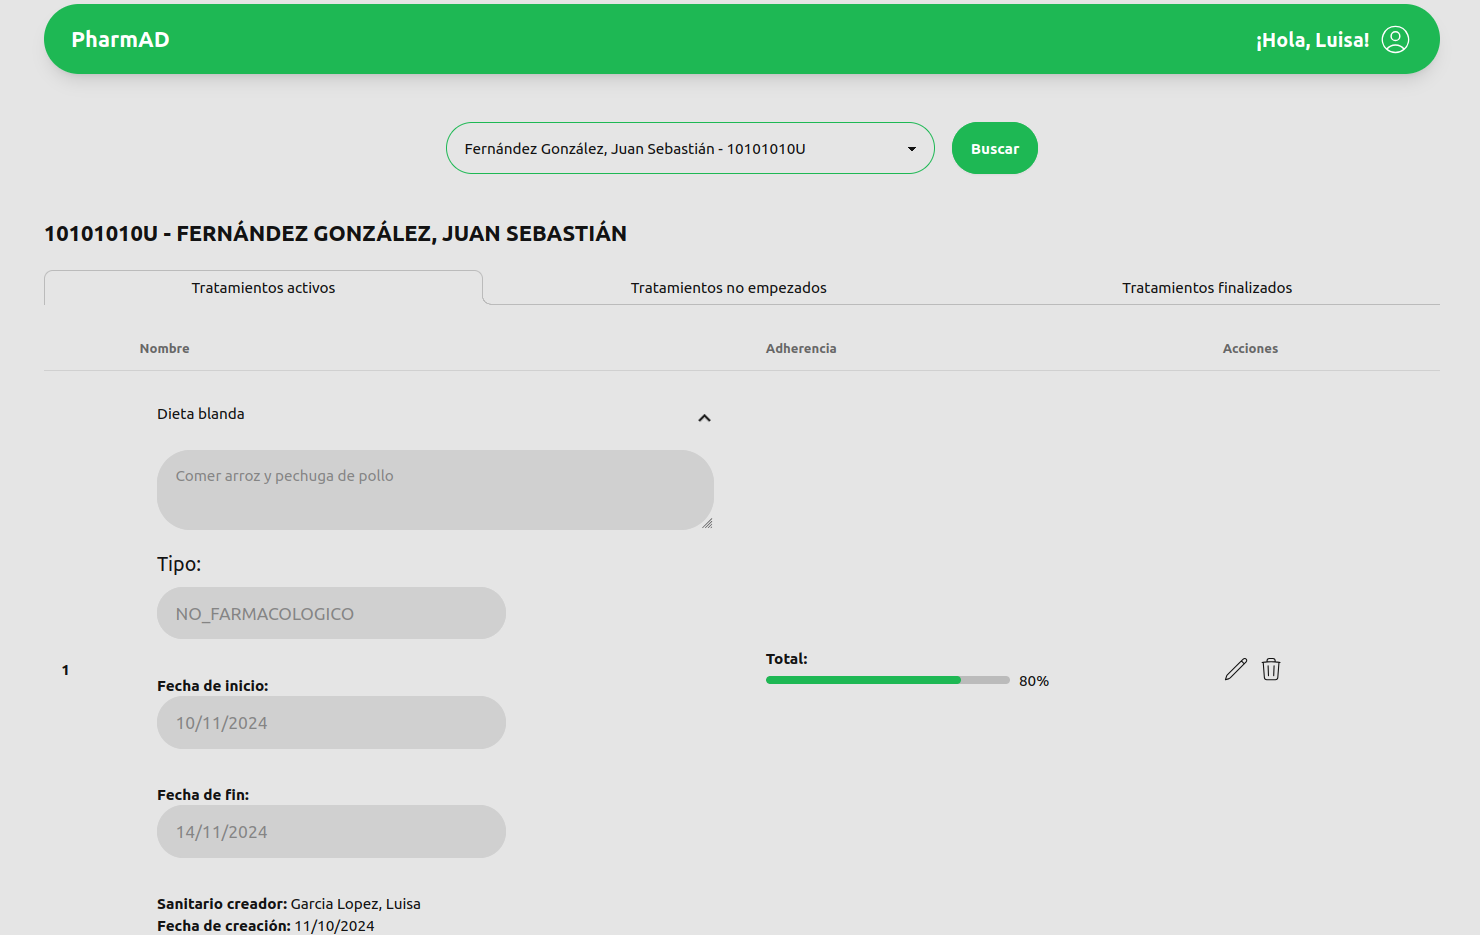
\includegraphics[width=0.9\textwidth]{imagenes/gestionarTratamientos.png}
	\caption{Vista de gestión de tratamientos para un farmacéutico.}
\end{figure}













%
%\input{capitulos/05_Diseno}
%
%\input{capitulos/06_Implementacion}
%
%\input{capitulos/07_Pruebas}
%
\chapter{Conclusiones}
El desarrollo de este proyecto ha culminado en la creación de una plataforma que integra un backend escalable y eficiente con un frontend interactivo y funcional, satisfaciendo plenamente todos los requisitos establecidos inicialmente. El sistema es capaz de gestionar de forma segura y efectiva información crítica de pacientes y personal sanitario en el contexto de una farmacia comunitaria. 

\section{Despliegue}
Durante el desarrollo del proyecto se tomó la decisión de mantener esta plataforma como exclusiva para el uso en las farmacias inscritas. Se trata de un soporte orientado a facilitar el trabajo del personal sanitario de las farmacias comunitarias, y la peculiaridad que lo caracteriza es que no todo el público, sin previo registro y alta como paciente de una farmacia, podría tener acceso. Esta característica proporciona una grado más de seguridad para proteger la información personal y médica de cada persona.

\section{Dificultades encontradas}
El proyecto ha enfrentado desafíos significativos, especialmente en lo referente a la configuración e integración de las diversas tecnologías utilizadas. La implementación de Docker Compose para gestionar PostgreSQL y pgAdmin, junto con la integración de Prisma y Fastify, requirió un esfuerzo para garantizar que todos los servicios se comunicaran correctamente y de manera segura. Asimismo, la implementación de controladores y rutas en Fastify, así como la validación de usuarios y permisos, presentó complejidades tanto técnicas como lógicas. Esto fue particularmente relevante durante el desarrollo de mecanismos de autenticación y autorización utilizando JSON Web Tokens (JWT) para controlar el acceso a los datos de los usuarios.

En el ámbito del frontend, la configuración de Astro y su integración con React añadieron niveles adicionales de complejidad, especialmente en la estructuración de componentes y la optimización del rendimiento de la interfaz de usuario. \\


\section{Conclusión final}
A nivel personal, la satisfacción con el resultado obtenido es alta. Gracias a todo el aprendizaje obtenido se podrán ampliar y mejorar todas las funcionalidades que ofrece la plataforma y realizar un despliegue real en el futuro.
%
%\chapter{Conclusiones y Trabajos Futuros}
%
%
%%\nocite{*}
\bibliographystyle{unsrt}
\bibliography{bibliography/biblio}\addcontentsline{toc}{chapter}{Bibliografía}
%
%
%\appendix
%\input{apendices/manual_usuario/manual_usuario}
%%\input{apendices/paper/paper}
%\input{glosario/entradas_glosario}
% \addcontentsline{toc}{chapter}{Glosario}
% \printglossary
\chapter*{}
\thispagestyle{empty}

\end{document}
